\def\year{2017}\relax
%File: formatting-instruction.tex
\documentclass[letterpaper]{article}
\usepackage{aaai17}
\usepackage{times}
\usepackage{helvet}
\usepackage{subfig}
\usepackage{amssymb}
\usepackage{enumitem}
\usepackage{amsmath}
\usepackage{pifont}
\usepackage{multirow}
\usepackage{hyperref}
\usepackage[table,xcdraw]{xcolor}
\usepackage[normalem]{ulem}
\useunder{\uline}{\ul}{}
\usepackage{courier}
\usepackage{graphicx}
\usepackage{epstopdf}
\usepackage{epsfig}
\usepackage{xr}
\usepackage{enumitem}

%\setlist{nosep} % dense lists with enumitem
 
\newcommand{\xmark}{\ding{55}}%
\newcommand{\starmark}{\ding{72}}%
\frenchspacing
\setlength{\pdfpagewidth}{8.5in}
\setlength{\pdfpageheight}{11in}
\pdfinfo{
/Title (Learning Topical Social Sensors)
/Author (Author1, Author2, Author3}
\setcounter{secnumdepth}{1}  

\renewcommand{\vec}[1]{\mathbf{#1}}

\newcommand{\eat}[1]{}
\newcommand{\rev}[1]{{\color{blue}{#1}}}

 \begin{document}
% The file aaai.sty is the style file for AAAI Press 
% proceedings, working notes, and technical reports.
%
\title{Learning Topical Social Sensors}
\author{Authors\\
Affiliations
}
\maketitle
\begin{abstract}
%!TEX root = icwsm2017_poster.tex

Twitter represents a massively distributed information source over a kaleidoscope of topics ranging from social and political events to entertainment and sports news.  While recent work has suggested that variations on standard classifiers can be effectively trained as topical filters~\cite{lin2011smoothing,yang2014large,magdy}, there remain many open questions about the efficacy of such classification-based filtering approaches.  For example, over a year or more after training, how well do such classifiers generalize to future novel topical content, and are such results stable across a range of topics?  Furthermore, what features and feature classes are most critical for long-term classifier performance?  To answer these questions, we collected a corpus of over 800 million English Tweets via the Twitter streaming API during 2013 and 2014 and learned topic classifiers for 10 diverse themes ranging from social issues to celebrity deaths to the ``Iran nuclear deal''.  The results of this long-term study of topic classifier performance provide a number of important insights, among them that (1) such classifiers can indeed generalize to novel topical content with high precision over a year or more after training and (2) simple terms and locations are the most informative feature classes (despite training on classes labeled via hashtags).  
%In summary, this work provides a long-term study of topic classifiers on Twitter that further justifies classification-based topical filtering approaches while providing insight into the feature properties most critical for topic classifier performance.
\end{abstract}

\section{Introduction}
%!TEX root = main.tex

\label{sec:introduction}

Social media sites such as Twitter present a double-edged sword for
users.  On one hand these sources contain a vast amount of novel and
topical content that challenge traditional news media sources in terms
of their timeliness and diversity.  Yet on the other hand they also
contain a vast amount of chatter and otherwise low-value content for most
users' information needs where filtering out irrelevant content is
extremely time-consuming.  Previous work~\cite{lin2011smoothing,yang2014large,magdy} 
has noted this need for topic-based filtering and has adopted a range
of variations on supervised classification techniques to build effective
topic filters.

While these previous approaches have augmented their respective topical classifiers with extensions
ranging from semi-supervised training to multiple stages of classification-based filtering to online tracking of foreground and background language model evolution, 
% --- all critical for state-of-the-art performance ---
we seek to analyze the lowest common denominator
of all of these methods, namely the performance of the underlying (vanilla) supervised 
classification paradigm.
Our fundamental research questions in this paper are hence focused on a longitudinal study
of the performance of such supervised topic classifiers.  
%taken a variety
%of approaches ranging from information retrieval and language models~\cite{lin2011smoothing}  
%to topic modeling~\cite{yang2014large} to supervised classification~\cite{magdy}.
For example, over a year or more after training, how well do such classifiers generalize to future novel topical content, and are such results stable across a range of topics?  Furthermore, what features, feature classes, and feature attributes are most critical for long-term classifier performance?  

To answer these questions, we collected a corpus of over 800 million English Tweets via the Twitter streaming API during 2013 and 2014 and learned topic classifiers for 10 diverse themes ranging from social issues to celebrity deaths to the ``Iran nuclear deal''.  We leverage ideas from~\cite{lin2011smoothing} for curating hashtags to define our 10 training topics and label
tweets for supervised training; however, we also curate a disjoint set of test hashtags %\emph{and use only these to label test data} (because training hashtags can be trivially memorized) 
to test true generalization performance of the topic filters to future novel content. 

We empirically show that two simple and efficiently trainable methods ---
logistic regression and naive Bayes --- generalize well to unseen
future topical content (including content with no hashtags) in terms
of their average precision (AP) and Precision@$n$ (for a range of
$n$) evaluated over long time-spans of typically one year or more.  
Furthermore, we show that terms and locations are among the most
useful features --- surprisingly more so than hashtags, even though
hashtags were used to label the data.  And perhaps even more
surprisingly, the number of unique hashtags and tweets by a user
correlates more with their informativeness than their follower or
friend count.  

In summary, this work\footnote{This is an extended and revised version of a preliminary conference report that was presented in~\cite{Iman2017}.} provides a longitudinal study of Twitter topic classifiers that further justifies supervised approaches used in existing work while providing detailed insight into feature properties critical for their performance.

%Twitter hosts lots of information, on average more than $2,200$ new tweets every second. This can get up to $3$ to $4$ times increase during large events such as tsunami. \footnote{\hyperref[]{https://blog.twitter.com/2011/the-engineering-behind-twitter-s-new-search-experience}}
%\begin{itemize}
%\item Twitter is a vast sensor of content generated by latent phenonema (e.g., flu, political sentiment, elections, environment).
%\item Learning topical social sensors (politicians in NY, road conditions in Toronto) -- very broad topics for which its hard to manually specify a useful query.
%\item But there is interesting topical content and wouldn't it be cool if we could learn a social sensor for a targeted topic?
%\item Key insight is that hashtags are topical and can be used to bootstrap a supervised learning system that as we will show generalizes well beyond the seed hashtags.
%\item Conclusion is a new way to build topical real-time feeds that are otherwise difficult to do with existing Twitter tools (???).
%\end{itemize}
%section{Learning Topical Social Sensors}

%Start off with the questions that we want to answer in this section:
%
%- How to evaluate, labeling (problem of no supervised labels for tweets, indirect via hashtags as topical surrogates, leads to question of hashtag curation)?
%
%- Which classification algorithm is best / most robust for learning topical social sensors?



%!TEX root = document.tex

%start with a clean argument then fill in details.  
%Motivation is mostly the same, 
%contributions are different... we combine recent ideas on learning social sensors 
%	(you need to cite / cover what these ideas are to indicate what you're combining / building on -- perhaps being clear to point out that no single paper did everything you are doing) and then claim that beyond a general performance analysis of the framework over a variety of topics and a long-term dataset (not done previously?) 
%a key objective of the work is to provide a comprehensive longitudinal feature analysis to investigate XXX

\COMMENT
{\color{red}
In this work, we coalesce recent ideas on learning social sensors for general topic detection. We expand these works to learn a generalizable supervised method with minimal user curation for detecting and ranking topical content over a variety of topics and on a long-term dataset. We believe that no earlier work covers all the aspects of the work presented here.
Earlier works discuss leveraging learning methodologies for detection of topical content from social media for general topics \citep{lin2011smoothing,yang2014large,magdy}. One of the key challenges of using learning methods for general topics and large number of tweets is automatic labeled data aquisition. To this purpose, \cite{lin2011smoothing} discuss automatic labeling of tweets by using one hashtag as topic proxy. \cite{magdy} use a user-defined query to label tweets and \cite{yang2014large} take a co-training approach based on embedded URLs in the tweet and tweet text to label tweets. We build and extend on \citep{lin2011smoothing}'s idea of automatic labeling of tweets, however we choose a \emph{set} of hashtags for each topic instead of a single hashtag which we will show to be imperative for evaluating generalization. To learn social sensors for general topic detection, \citep{lin2011smoothing} use information retrieval method (language models), \cite{yang2014large} take advantage of topic modeling techniques and \cite{magdy} apply SVM classifier. Here, we leverage more than one supervised learning method for the purpose of detection and ranking of topical content. We present a unique method for splitting hashtags and Twitter data that encourages generalization to new unseen future content. 
%Recently, \citep{lin2011smoothing,yang2014large,magdy} have explored use of social media sensors for detection and/or tracking of general topics from Twitter. One of the key challenges on dealing with general topics and large number of tweets is automatic labeled data aquisition. \cite{lin2011smoothing} discusses automatic labeling of tweets by using one hashtag as topic proxy. \cite{magdy} uses a user-defined query to label tweets and \cite{yang2014large} takes a co-training approach based on embedded URLs in the tweet and tweet text to label tweets. We build and extend on \citep{lin2011smoothing}'s idea of automatic labeling of tweets, however we choose a set of hashtags for each topic instead of a single hashtag which we will show to be imperative for evaluating generalization. To learn social sensors for general topic detection, \citep{lin2011smoothing} uses information retrieval method (language models), \cite{yang2014large} take advantage of topic modeling techniques and \cite{magdy} applies SVM classifier. Here, we leverage various supervised learning methods for the purpose of detection and ranking of topical content. However, we present a unique method for splitting hashtags and Twitter data that encourages generalization to new unseen future content. 
%The methodologies mentioned in the literature use various sets of feature including hashtags, unigrams, bigrams, mentions, users, byte 4grams. We extract the main features of hashtags, mentions, users, unigrams. In addition, we add location as another set of features which we show later in feature analysis that location is the second most important feature for detection of topical content and some of the topics are quite localized geographically. To address general topic detection from social media, \cite{lin2011smoothing} uses information retrieval method (language models), \cite{yang2014large} take advantage of topic modeling techniques and \cite{magdy} uses SVM classifier. Here, we leverage various supervised learning methods for the purpose of detection and ranking of topical content. However, we present a unique method for splitting hashtags and Twitter data that encourages generalization to new unseen future content. 
}
\ENDCOMMENT

\section{Related Work}
%!TEX root = main.tex
% Scott's outline
%
% EU Social Sensor project: what to say?  Many works integrated
%   into following text, but none specifically learning topical sensors
%   from supervised labels.
%
% Trending topics: learning but not supervised
%
% RT recommendation: RTs are personalized but not topical
%
% Specific events: predicting earthquakes.
%
% Friend sensor: friendship paradox, focusing of friends-only, no supervised
%                training for a topic, just trying to pick informative users
%                however: our work suggests users are least important features
%                (Figure 2)

%%%%% TRACKING GENERAL TOPICS
% TODO for Scott: Need to rewrite in a more retrospective manner.
%                 Should this go as the first point in related work?
\vspace{2mm}
\subsection*{Twitter Topic Classification} 

Topic classification for social media aims to detect and track general topics such as "Baseball" or "Fashion".  In previous work, researchers have collected labeled data either by using a single hashtag for each topic~\citep{lin2011smoothing}, a user-defined query for each topic~\citep{magdy}, or co-training based on the URLs and text of the tweet \citep{yang2014large}.
% \cite{lin2011smoothing} leverages language models to train models using unigrams and bigrams, \cite{magdy} applies SVM classifier on extracted hashtags, unigrams, users and mentions as features, and \cite{yang2014large} defines the problem as topic modeling of tweets. 
We expand on \citep{lin2011smoothing}'s work and use a set of hashtags instead of a single hashtag.  Similarly, we extract features consisting of hashtags, mentions, unigram terms, and authors as done in this prior work, but also add location as another feature, which has shown to be the second most important feature for topic classification after unigram terms.
Furthermore, we provided a novel learning and evaluation paradigm based on splitting both the data and hashtags along temporal boundaries to generate train, validation and test datasets in order to evaluate long-term generalization of trained topic classifiers.  In contrast, we remark that \citep{lin2011smoothing} only evaluated over 1 week, \citep{magdy} over 4 days,
and \citep{yang2014large} did not explicitly mention the data duration or that their study was intended to assess long-term performance.  Hence these previous studies do not permit one to assess the long-term topic classification performance of topic classifiers for Twitter as intended by the 2 year longitudinal study performed in this article.

% there are many fine-grain but important differences between previous works and this work with the most important ones being:
% \begin{enumerate}
% \item We analyzed long-term sensor performance on detecting topical content over two years of Twitter data and across a variety of topics.
% \item We provide a novel and clear framework for splitting hashtags to train, validation and test in a way ensuring generalization to long term unseen future content.
% \item We present ranking in addition to correct classification while none of the other works provide ranking.
% \item We deliver a comprehensive longitudinal study on features and their attributes over two years of tweets that supports our insights for learning and relevance of features to topicality while these works had little or none analysis over their features.
% \item We extract \textit{Location} as one of the features which none of these works do and as we show in our feature analysis, \textit{Location} is the second most important feature beating even hashtags in terms of correlation with topicality.

\subsection*{Related Applications of Classifiers for Social Media} 

Aside from highly related work on supervised topic classifiers for Twitter~\cite{lin2011smoothing,yang2014large,magdy} that motivated this study as discussed previously, there are many other uses of classifiers for social media.  While we
argue no prior work has performed a longitudinal analysis of supervised Twitter topical 
classifiers as done in this article, these alternative applications of classifiers for social media may broadly benefit from the insights gained by our present study.  We cover these related uses below along with important differences with the present work, divided into the following four subareas: (1) trending topic detection, (2) tweet recommendation, (3) friend
sensors, and (4) specific event detection such as earthquake or
influenza sensors.   
%In the following, we explain why each of these four areas is different from
%the social sensor learning work proposed here.

\vspace{2mm}
\noindent {\bf Trending Topic Detection} represents one of the most popular
types of topical tweet detector and can be subdivided into many categories.  The
first general category of methods define trends as topically coherent
content and focus on clustering across lexical, linguistic, temporal
and/or spatial
dimensions~\cite{petrovic,ishikawa,murata,becker,tweetmotif,wangLee}.
%\cite{wei} proposed a
%graphical model to discover latent events clustered in the spatial,
%temporal and lexical dimensions, while \cite{yamamoto} focused on the
%task of multi-label classification of tweets into living aspects such
%as eating.
The second general category of methods define trends as temporally
coherent patterns of terms or keywords and focus largely on detecting
bursts of terms or
phrases~\cite{mathioudakis,cuiZhang,zhaoSports,nichols,aiello}.
% I don't know that this means... aren't all of the above methods user-defined
% criteria as well? -SPS
%
%The third category, query-based methods, focuses on the hypothesis that trending
%topics can be detected by measuring user defined
%criteria \cite{albakour,sakakiDrive}.
The third category of methods extends the previous categories by
additionally exploiting network structure properties~\cite{budak}.
Despite this important and very active area of work that can be
considered a type of topical tweet detector, trending topic detection is
intrinsically unsupervised and not intended to detect targeted topics.
In contrast, the work in this article is based on supervised learning of
a specific topical tweet detector trained on the topical set of
hashtags provided by the user.

% From EU Social Sensor Project...
%
% NOTE: Whoa... this is everything yet nothing... not worth discussing. -SPS
%The final category, hybrid method
%of \cite{diplaris} introduced concept of Dynamic Social Containers in
%this work to take advantage of aggregation of mining both the
%structure, content, and multimedia data to index and provide
%personalized, context-aware search. In this work, the authors defined
%social sensor as analyzing the dynamic and massive amount of
%information provided by user with the purpose of extracting unbiased
%trending topics and events in addition to using social connections for
%recommendation.

% From EU Social Sensor Project...
%
% This is just a TF-IDF term-based method, not worth a separate discussion
%With the purpose of comparison of methods, \cite{aiello} evaluated six
%trending topic detection methods on three Twitter datasets differing
%in time scale and topic churn rate. The authors conclude that natural
%language processing techniques perform well on focused
%topics. However, techniques mining temporal distribution of concepts
%are needed to handle more heterogeneous streams.

% Zahra: trending topics are unsupervised... we're supervised. -SPS
% 
%However, trending topics detection methods are not targeted. Our
%method differs from trending topic detection methods in that we are
%focusing on a set of topics that cannot necessarily be detected using
%bursts.Thus, trending topics detection methods are of limited
%relevance to the work presented hereinafter.

\vspace{2mm}
\noindent {\bf Tweet Recommendation} represents an alternate use of
tweet classification and falls into two broad categories: personalized or
content-oriented recommendation and retweet recommendation.  For the
first category, the objective of personalized recommendation is to
observe a user's interests and behavior from their user profile,
sharing or retweet preferences, and social relations to generate
tweets the user may like~\cite{Yan,chen}.  The objective of
content-oriented recommendation is to use source content (e.g., a news
article) to identify and recommend relevant tweets (e.g., to allow
someone to track discussion of a news article)~\cite{Krestel}.  For
the second category, there has been a variety of work on retweet
prediction that leverages retweet history in combination with
tweet-based, author-based, and social network features to predict
whether a user will retweet a given
tweet~\cite{can,xu,petrovicOsborne}.  Despite the fact that all of
these methods recommend tweets, they --- and recommendation methods in
general --- are not focused on a specific topic but rather on
predicting tweets that correlate with the preferences of a specific
user or that are directly related to specific content.  Rather the
focus with learning topical classifiers is to learn to predict for
a broad theme (independent of a user's profile) in a way that
generalizes beyond existing labeled topical content to novel future
topical content.

%Another set of studies have moved towards creating more generalizable
%methods. Using a dataset of 55,000 news articles and 121,000
%tweets, \cite{Krestel} compared four different methods of language
%model, topic model, logistic regression, and boosting, to evaluate
%recommended tweets for a given news article.. \cite{Yan,chen} also
%focused on tweet recommendation. Their methods considered the user’s
%twitter profile, including tweet and retweet history, and social
%relations as features. Coupled with tweet popularity, the methods are
%able to generate tweet recommendations. With the purpose of photo
%recommendation on social media websites, \cite{chiarandini} analyzed
%the user logs of pageviews, navigation patterns between
%photostreams. The authors used collaborative filtering method and
%built a stream transition graph to analyze common stream topic
%transitions to this end.

%On retweet prediction, \cite{can,xu,petrovicOsborne} used
%classification-based approaches using tweet-based and author-based
%features. However, \cite{can} took advantage of visual cues from
%images linked in the tweets, and \cite{xu} employed social-based
%features in addition to tweet author-based features. Different from
%the other two works, \cite{xu} performed the analysis from the
%perspective of individual users. \cite{petrovicOsborne} worked on
%retweet prediction of real-time tweeting with online learning
%algorithms and claimed that performance is dominated by social
%features, but that tweet features add a substantial boost. These
%studies showed that temporal features have a stronger effect on
%messages with low and medium volume of retweets compared to highly
%popular messages, and user activity features can further improve the
%performance marginally.

%%%%% TARGETED SPECIFIC TOPIC DETECTION
\vspace{2mm}
\noindent {\bf Specific Event Detection} builds topical tweet detectors 
as we do in this work but focuses on highly specific events 
such as disasters or epidemics.  For the use case of earthquake
detection, an SVM can be trained to detect earthquake events
and coupled with a Kalman filter for localization~\cite{sakakiEq2}.
%
%% Decriptive studies irrelevant to building social sensors. -SPS
%
%Whereas the above works addressed exploiting the detection of crisis
%events, the following works focused on descriptive studies on
%disaster. The studies discuss the behavior of Twitter users during a
%crisis \cite{vieweg,cheong,starbird} and do not address exploiting
%detection of crisis events. The studies investigated the use of social
%media during a crisis in order to identify information propagation
%properties, the social behavior of users (their retweeting behavior),
%information contributing to situational awareness, and the active
%players in communicating information. The behavioral information
%gleaned from these studies is exploited in this work to aid in the
%development of social sensors for detection of topics.
%
In another example use case to detect health epidemics such as
influenza, researchers build purpose-specific classifiers targeted to
this specific epidemic~\cite{culotta,aramaki}, e.g, by exploiting
knowledge of users' proximity and friendship along with the contageous
nature of influenza~\cite{sadilek}.  While these targeted event
detectors have the potential of providing high precision event
detection, they are highly specific to the target event and do not
easily generalize to learn arbitrary topic-based classifiers
for Twitter as analyzed in this work.

\vspace{2mm}
\noindent {\bf Friend Sensors} 
are a fourth and final class of social sensors intended for early
event detection~\cite{sandy,garcia} by leveraging the concept of the
``friendship paradox''~\cite{feld}, %~\footnote{On average, most people have
%fewer friends than their friends have.}),
to build user-centric social sensors.  We note that our topical classifiers 
represent a \emph{superset} of friend sensors since our work
includes author features that the predictor may learn to use if this
proves effective for prediction.  However, as shown in our feature
analysis, user-based features are among the least informative feature
types for our topical classifier suggesting that general topical 
classifiers can benefit from a wide variety of features well beyond those of
author features alone.





%In this regard, \citeauthor{garcia} provided a method for
%choosing sensor groups from friends of random sets of users to find
%more central individuals in order to enforce early detection. The
%central assumption made in this work is that a sensor group represents
%more central individuals, and individuals at the center of a network
%are more likely to become infected than randomly-chosen members of the
%population. As a result, \citep{garcia} argued that this selection
%process of sensor groups helps in the early detection of outbreaks.

%%%%%%% SOCIAL SENSOR PROJECT
%% NOTE: the citations below have been integrated into the text above... separate back out?
%
%Social sensor project \footcite{http://www.socialsensor.eu/} 
%\citep{aiello} compared six trending topic detection methods on three Twitter datasets differing in time scale and topic churn rate. The authors conclude that natural language processing techniques perform well on focused topics. However, techniques mining temporal distribution of concepts are needed to handle more heterogeneous streams.
%\citep{diplaris} defines social sensor as analyzing the dynamic and massive amount of information provided by user with the purpose of extracting unbiased trending topics and events in addition to using social connections for recommendation. The authors introduce concept of Dynamic Social Containers in this work to take advantage of aggregation of mining both the structure, content, and multimedia data to index and provide personalized, context-aware search.
%With the purpose of photo recommendation on social media websites, \citep{chiarandini} analyzed the user logs of pageviews, navigation patterns between photostreams. The authors used collaborative filtering method and built a stream transition graph to analyze common stream topic transitions to this end.

%%%%%%%%%%%%%%% TWITTER CURRENT SEARCH METHOD %%%%%%%%%%%%%%%%%
%% UNUSED
%\iffalse
%
%Twitter model: reverse indexes was built in MySQL, leveraging its concurrent transactions and B-tree data structures to support indexing and searching partitioned across multiple databases. Earlybird, a real-time reverse index based on Lucene, gave much better performance and memory efficiency than MySQL for real-time search. 
%"There is a lot of information on Twitter — on average, more than 2,200 new Tweets every second! During large events, for example the \#tsunami in Japan, this rate can increase by 3 to 4x. Often, users are interested in only the most memorable Tweets or those that other users engage with. In our new search experience, we show search results that are most relevant to a particular user. So search results are personalized, and we filter out the Tweets that do not resonate with other users."
%
%Supporting personalized search, they needed three types of signal: Static signals at indexing time, Resonance signals updated over time, Information about the searcher at search time. At indexing time, tweets are annotated with static information about the user and the language of the tweet's text. Dynamic updates, such as users' interactions with tweets are made over time. At query time, user's social graph is passed along the user's query. A specialized ranking function is used to combine relevance signals and the social graph for computing personalized relevance score for each tweet. The results consists of highest-ranking, most-recent tweets. The ranking function accesses the social graph and uses knowledge about the relationship between the searcher and the author of a tweet during ranking.
%\fi
%%%%%%%%%%%%%%%%%%%%%%%%%%%%%%%%%%%%%%%%%%%%%%%%%%%%%%


\section{Learning Topical Social Sensors}
\label{sec:lss}
%!TEX root = icwsm2017_poster.tex

% This section covers the *formal* framework for learning topical social sensors

% =====================
% What are we doing?  
% (1) Formal problem setup and notation definitions.  Corpus of documents, features, labels, classification problem definition (for a generic classifier).
% (2) How we label data.
% (3) How we train (validation set critical for hyperparameters, what metric used for selection?).
% Note that formal performance evaluation provided in experimental section.
% =====================

% (1) Formal problem setup and notation definitions.  Corpus of documents, features, labels, classification problem definition (for a generic classifier).
%TODO: Formal learning framework.
Our objective is to build a binary classifier that can label
a previously unseen tweet as topical (or not) by training on 
topically labeled historical tweets.  
%
%Formally, 
%given an arbitrary tweet $d$ (a document in text classification parlance) 
%and a set of topics $T = \{
%t_1,\ldots,t_K\}$, we wish to train a scoring function $f^t: D \rightarrow \mathbb{R}$
%for topic $t \in T$ over a subset of labeled training tweets from $D = \{
%d_1,\ldots,d_N \}$.  Each $d_i \in D$ has a boolean feature vector 
%$(d_i^1,\ldots,d_i^M) \in \{0,1\}^M$.  A boolean function $t : D \rightarrow \{
%0,1 \}$ indicates whether the tweet $d_i$ is topical (1) or not
%(0).  In an ideal scenario, we could train for topic $t$ 
%so that $\forall d_i \; f^t(d_i) = t(d_i)$ --- our scoring
%function (or more generally some threshold on it) agrees perfectly with the topic
%labels of all tweets.  
%
%A critical bottleneck for learning targeted topical social classifiers 
%is to achieve sufficient supervised content labeling.  With data
%requirements often in the thousands of labels to ensure effective
%learning and generalization over a large candidate feature space (as
%found in social media), manual labeling is simply too time-consuming
%for many users, while crowdsourced labels are both costly and prone to
%misinterpretation of users' information needs.  Fortuitously, hashtags
%have emerged in recent years as a pervasive topical proxy on social
%media sites --- hashtags originated on IRC chat, were adopted later
%(and perhaps most famously) on Twitter, and now appear on other social
%media platforms such as Instagram, Tumblr, and Facebook.  
%
Following
the approach of~\cite{lin2011smoothing}, for each topic $t \in T$, we leverage a (small) set of
user-curated topical hashtags $H^t$ to efficiently provide a large number of
supervised topic labels for social media content.  
%Next we provide
%a procedure for labeling data with $H^t$ for training and validation.
%Following this, we proceed to train
%supervised classification and ranking methods to learn topical content
%from a large feature space (e.g., this feature space
%includes terms, hashtags, mentions, authors and their locations). The
%training process involves two steps:
%\begin{enumerate}
%\item {\bf Temporally split train and validation using $H^t$:}
As standard for machine learning methods, we divide our training data into
train and validation sets --- the latter for hyperparameter tuning to control
overfitting and ensure generalization to unseen data.  
As a critical insight for topical generalization where we view correct classification 
of tweets with \emph{previously unseen topical hashtags} as a proxy for topical generalization, 
we \emph{do not} simply
split our data temporally into train, validation, and test sets and label both with \emph{all} 
hashtags in $H^t$.  \emph{Instead},
we split $H^t$ into three disjoint sets $H^t_\mathrm{train}$, $H^t_\mathrm{val}$, and 
$H^t_\mathrm{test}$ 
according to two time stamps $t^\mathrm{val}_\mathrm{split}$ and $t^\mathrm{test}_\mathrm{split}$ for topic $t$ and the first usage time stamp 
$h_\mathrm{time*}$ of each hashtag $h \in H^t$.  In short, all hashtags $h \in H^t$ with
$h_\mathrm{time*} < t^\mathrm{val}_\mathrm{split}$ are used to generate positive labels in the training data, those with $h_\mathrm{time*} \geq t^\mathrm{test}_\mathrm{split}$ are used to generate positive labels in the test data and the remainder are used to label the validation data.

%To achieve this effect formally, we define the following:
%\begin{align*}
%H^t_\mathrm{train} & = \{ h | h \in H^t \land h_\mathrm{time*} <    t_\mathrm{split} \} ,  \\
%H^t_\mathrm{val}   & = \{ h | h \in H^t \land h_\mathrm{time*} \geq t_\mathrm{split} \} .
%\end{align*}
%Once we have split our hashtags into training and validation sets
%according to $t_\mathrm{split}$, we next proceed to temporally split
%our training documents $D$ into a training set $D^t_\mathrm{train}$ and a validation set
%$D^t_\mathrm{val}$ for topic $t$ based on the posting
%time stamp $d_{i,\mathrm{time*}}$ of each tweet $d_i$ as follows: 
%%ormally, given $H^t$, we
%%can label each document $d_i$ (containing positive features $D_i^+$) as follows:
%\begin{align*}
%D^t_\mathrm{train} & = \{ d_i | d_i \in D \land d_{i,\mathrm{time*}} <    t_\mathrm{split} \} ,  \\
%D^t_\mathrm{val}   & = \{ d_i | d_i \in D \land d_{i,\mathrm{time*}} \geq t_\mathrm{split} \} .
%\end{align*}
%Next we define the set of positively occurring features for a document
%$d_i$ formally as $D_i^+ = \{ j | d_i^j=1 \}_{j=1\ldots M}$ and note that
%$D_i^+$ may include feature IDs for the content of $d_i$ (e.g., terms and, importantly, 
%hashtags) as well as its meta-data (e.g., author, location).
%Then to label both the train and validation data sets $D^t_\mathrm{train}$ and $D^t_\mathrm{val}$, 
%we use the respective
%hashtag sets $H^t_\mathrm{train}$ and $H^t_\mathrm{val}$ for generating
%the topic label for a particular tweet $t(d_{i}) \in \{0,1\}$ as follows:
%\begin{align*}
%t(d_{i}) & =
%  \begin{cases}
%    1: \exists_{h \in H^t_\mathrm{train}} \; h \in D_i^+ \land d_{i} \in D^t_\mathrm{train} \\
%    1: \exists_{h \in H^t_\mathrm{val}}   \;\;\; h \in D_i^+ \land d_{i} \in D^t_\mathrm{val}   \\
%    0: \mathrm{otherwise}
%  \end{cases} .
%\end{align*}

%To recap the methodology, we specify a set of hashtags as a proxy for a topic.  We split
%those hashtags into train and validation sets according to a time of first usage and fixed time point.
%We split the tweet data into train and validation sets according to the same fixed time point.
%Finally, we label a tweet in the train (validation) data set as positive if it contains
%a hashtag in the train (validation) hashtag set.  

The critical insight here is that we not only partition the train, validation, and test data 
temporally, but we also divide the hashtag labels temporally and label each data partition with
an entirely disjoint set of topical hashtags.
%Selection of a set of documents and temporally splitting them into
%train and validation documents. The split is based on a split-time
%defined on hashtag set $H^{t}$ to preserve enough number of hashtags
%in train and validation sets.
The purpose behind this training and validation data split
and labeling is to ensure that learning hyperparameters are tuned so as
to prevent overfitting and maximize generalization to unseen topical
content (i.e., new hashtags).
We remark that a classifier that simply
memorizes training hashtags will fail to correctly classify the validation data except in 
cases where a tweet contains both a training and validation hashtag.  

Next we proceed to train our classifier and  
%scoring function $f^t$ on $D^t_\mathrm{train}$ and
select hyperparameters to optimize Average Precision (AP)~\cite{manning_ir} (a ranking
metric) on the validation data (and hashtag labels).
Because all of our classifiers provide a real-valued score (e.g., logistic regression
provides the probability of the class), the classifiers can be used to rank.
In our results, we report final evaluations on the held-out test data with their own
disjoint set of topical hashtag labels.

%Analogously to train and validation data, test data is generated the same way, but 
%we omit formal notation (identical to the above) in order to reduce clutter.
%Test data has its own time stamp ($> t_\mathrm{split}$), its own set of
%temporally disjoint data, and its own set of hashtags 
%temporally disjoint from the training and validation data; this is done in order to evaluate
%generalization performance of the learned classifier on future data with topical hashtags
%not seen during training.    
%With train, validation, and testing data defined along with the training methodology,
%it remains now to empirically evaluate and analyze classifier performance, 
%described next.


\section{Data Description}
\label{sec:datasetStatistics}
%%%%%%%%%%%%%%%%%%%%%%%%%%%%%%%%%%%%%%%%%%%%%%%%%%%%%%%%%%%%%%%%%%%%%%%%%%%
\begin{figure*}[t!]
\centering
\begin{tabular}{ccc}
\begin{tabular}{ccc}
\subfloat[Fig:][Human Caused Disaster]{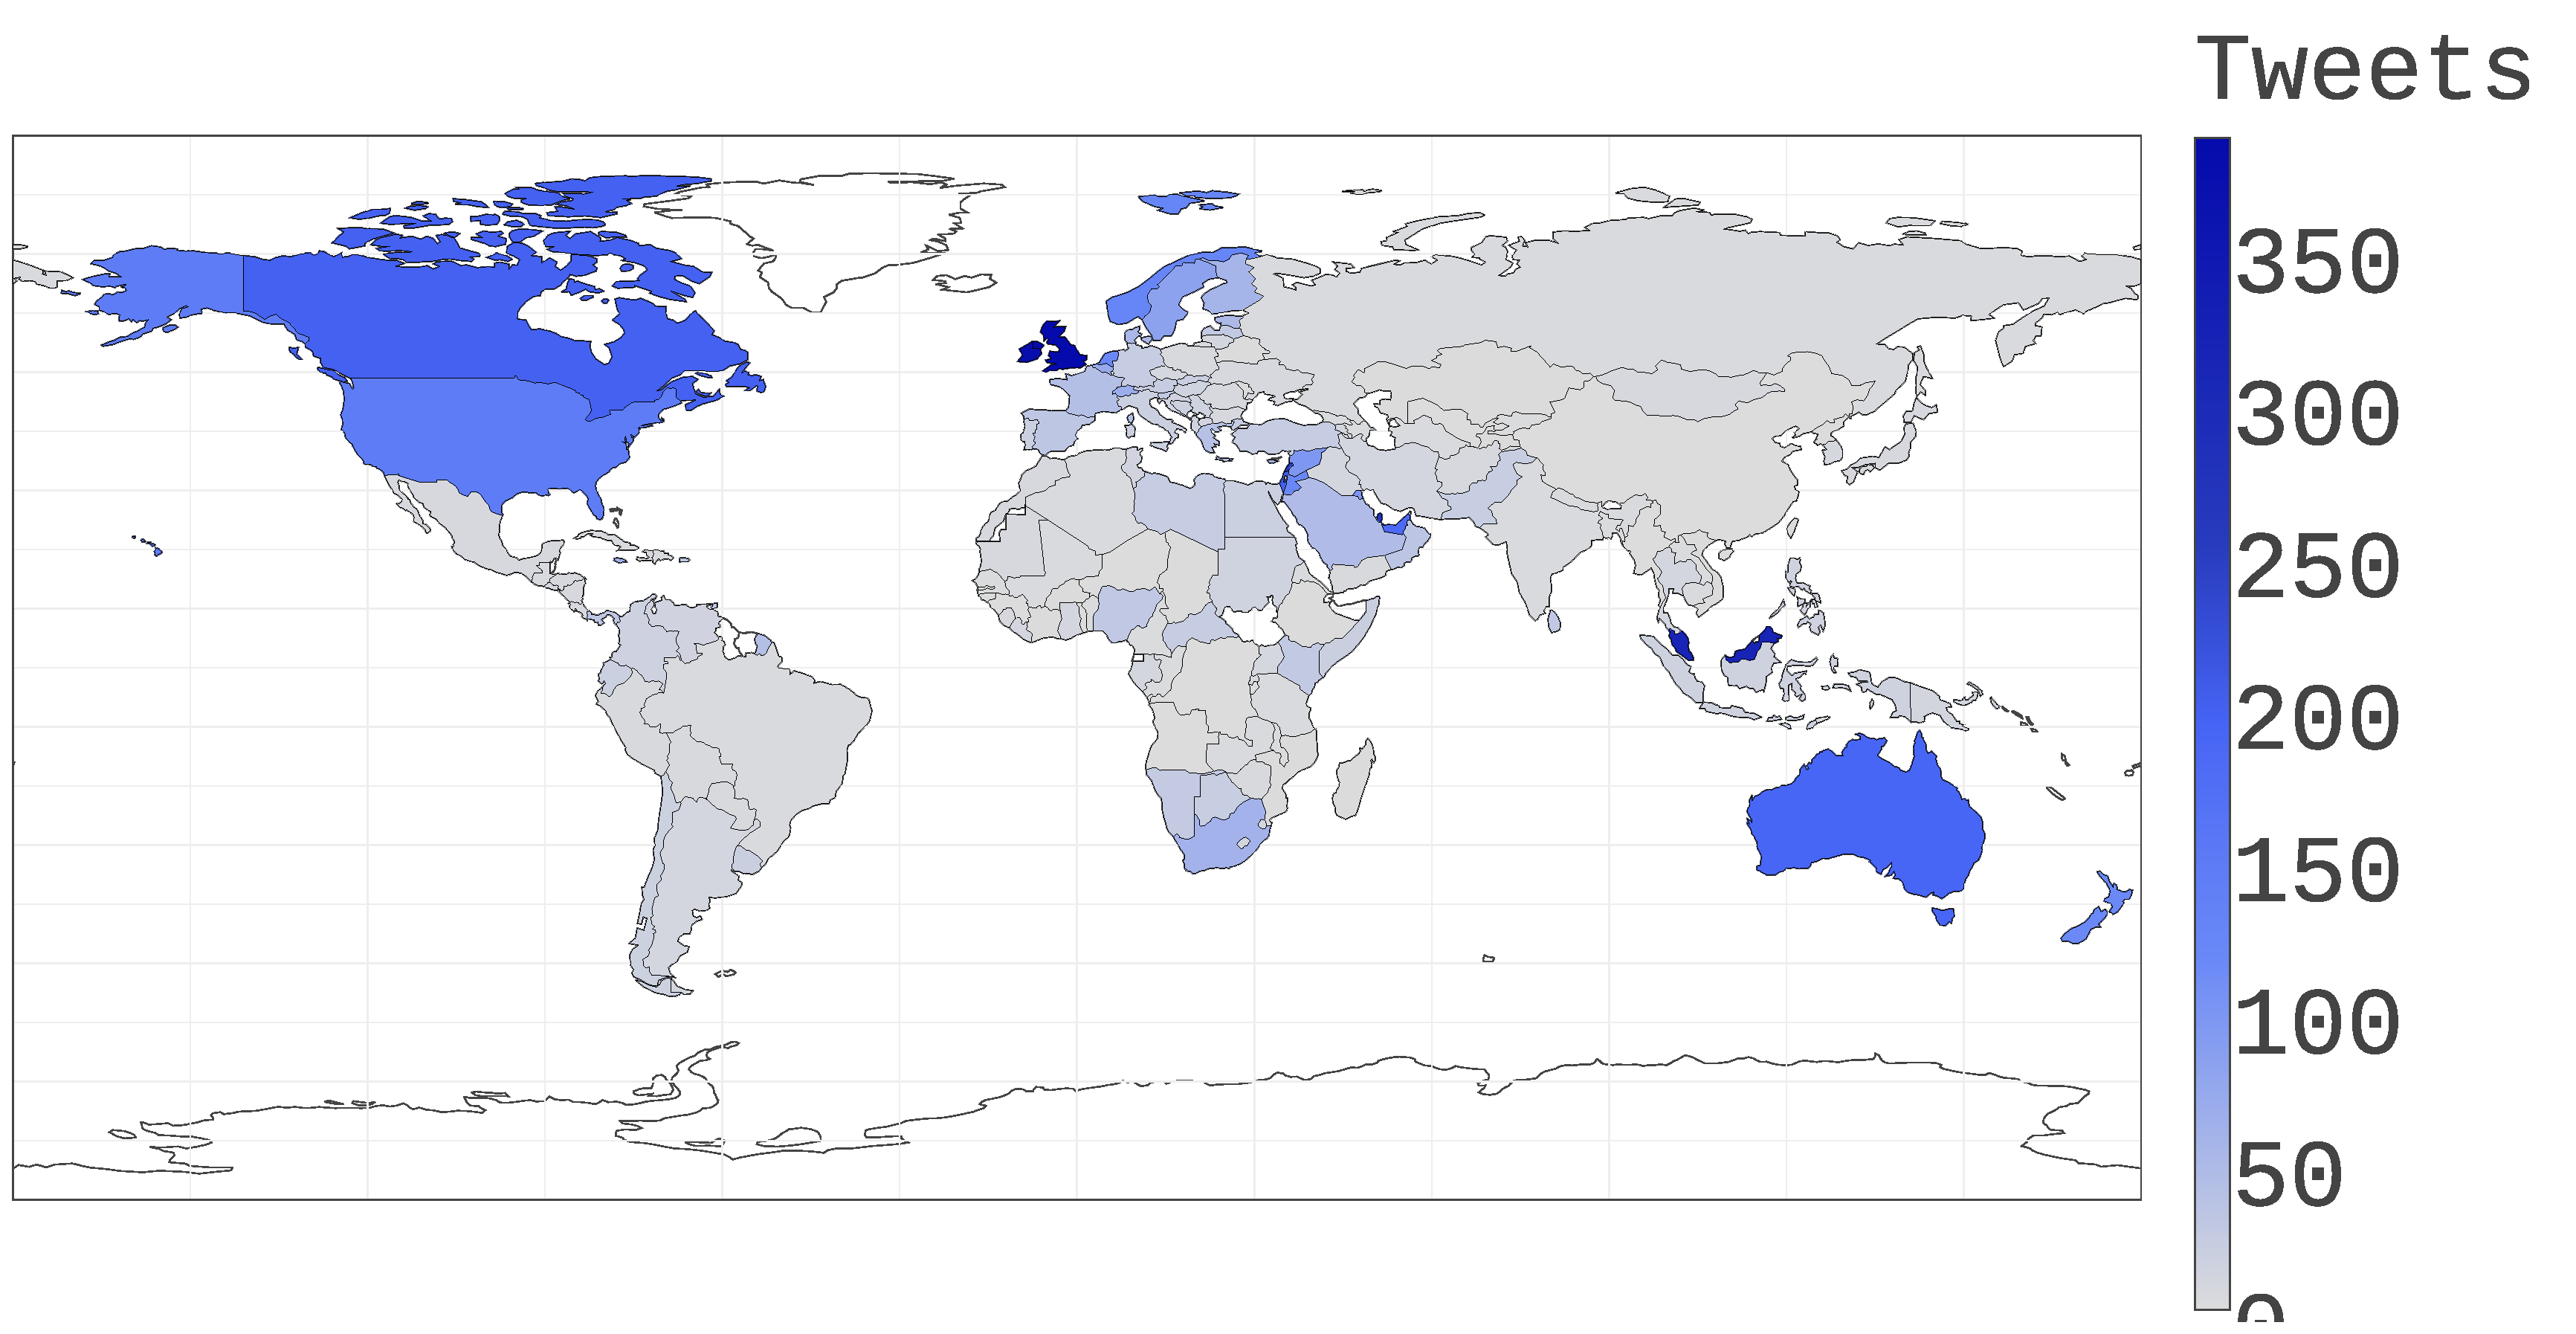
\includegraphics[width=5.3cm]{images/location/world/socialsensor-world-HumanCausedDisaster_location.eps}}
\subfloat[Fig:][Iran Deal]{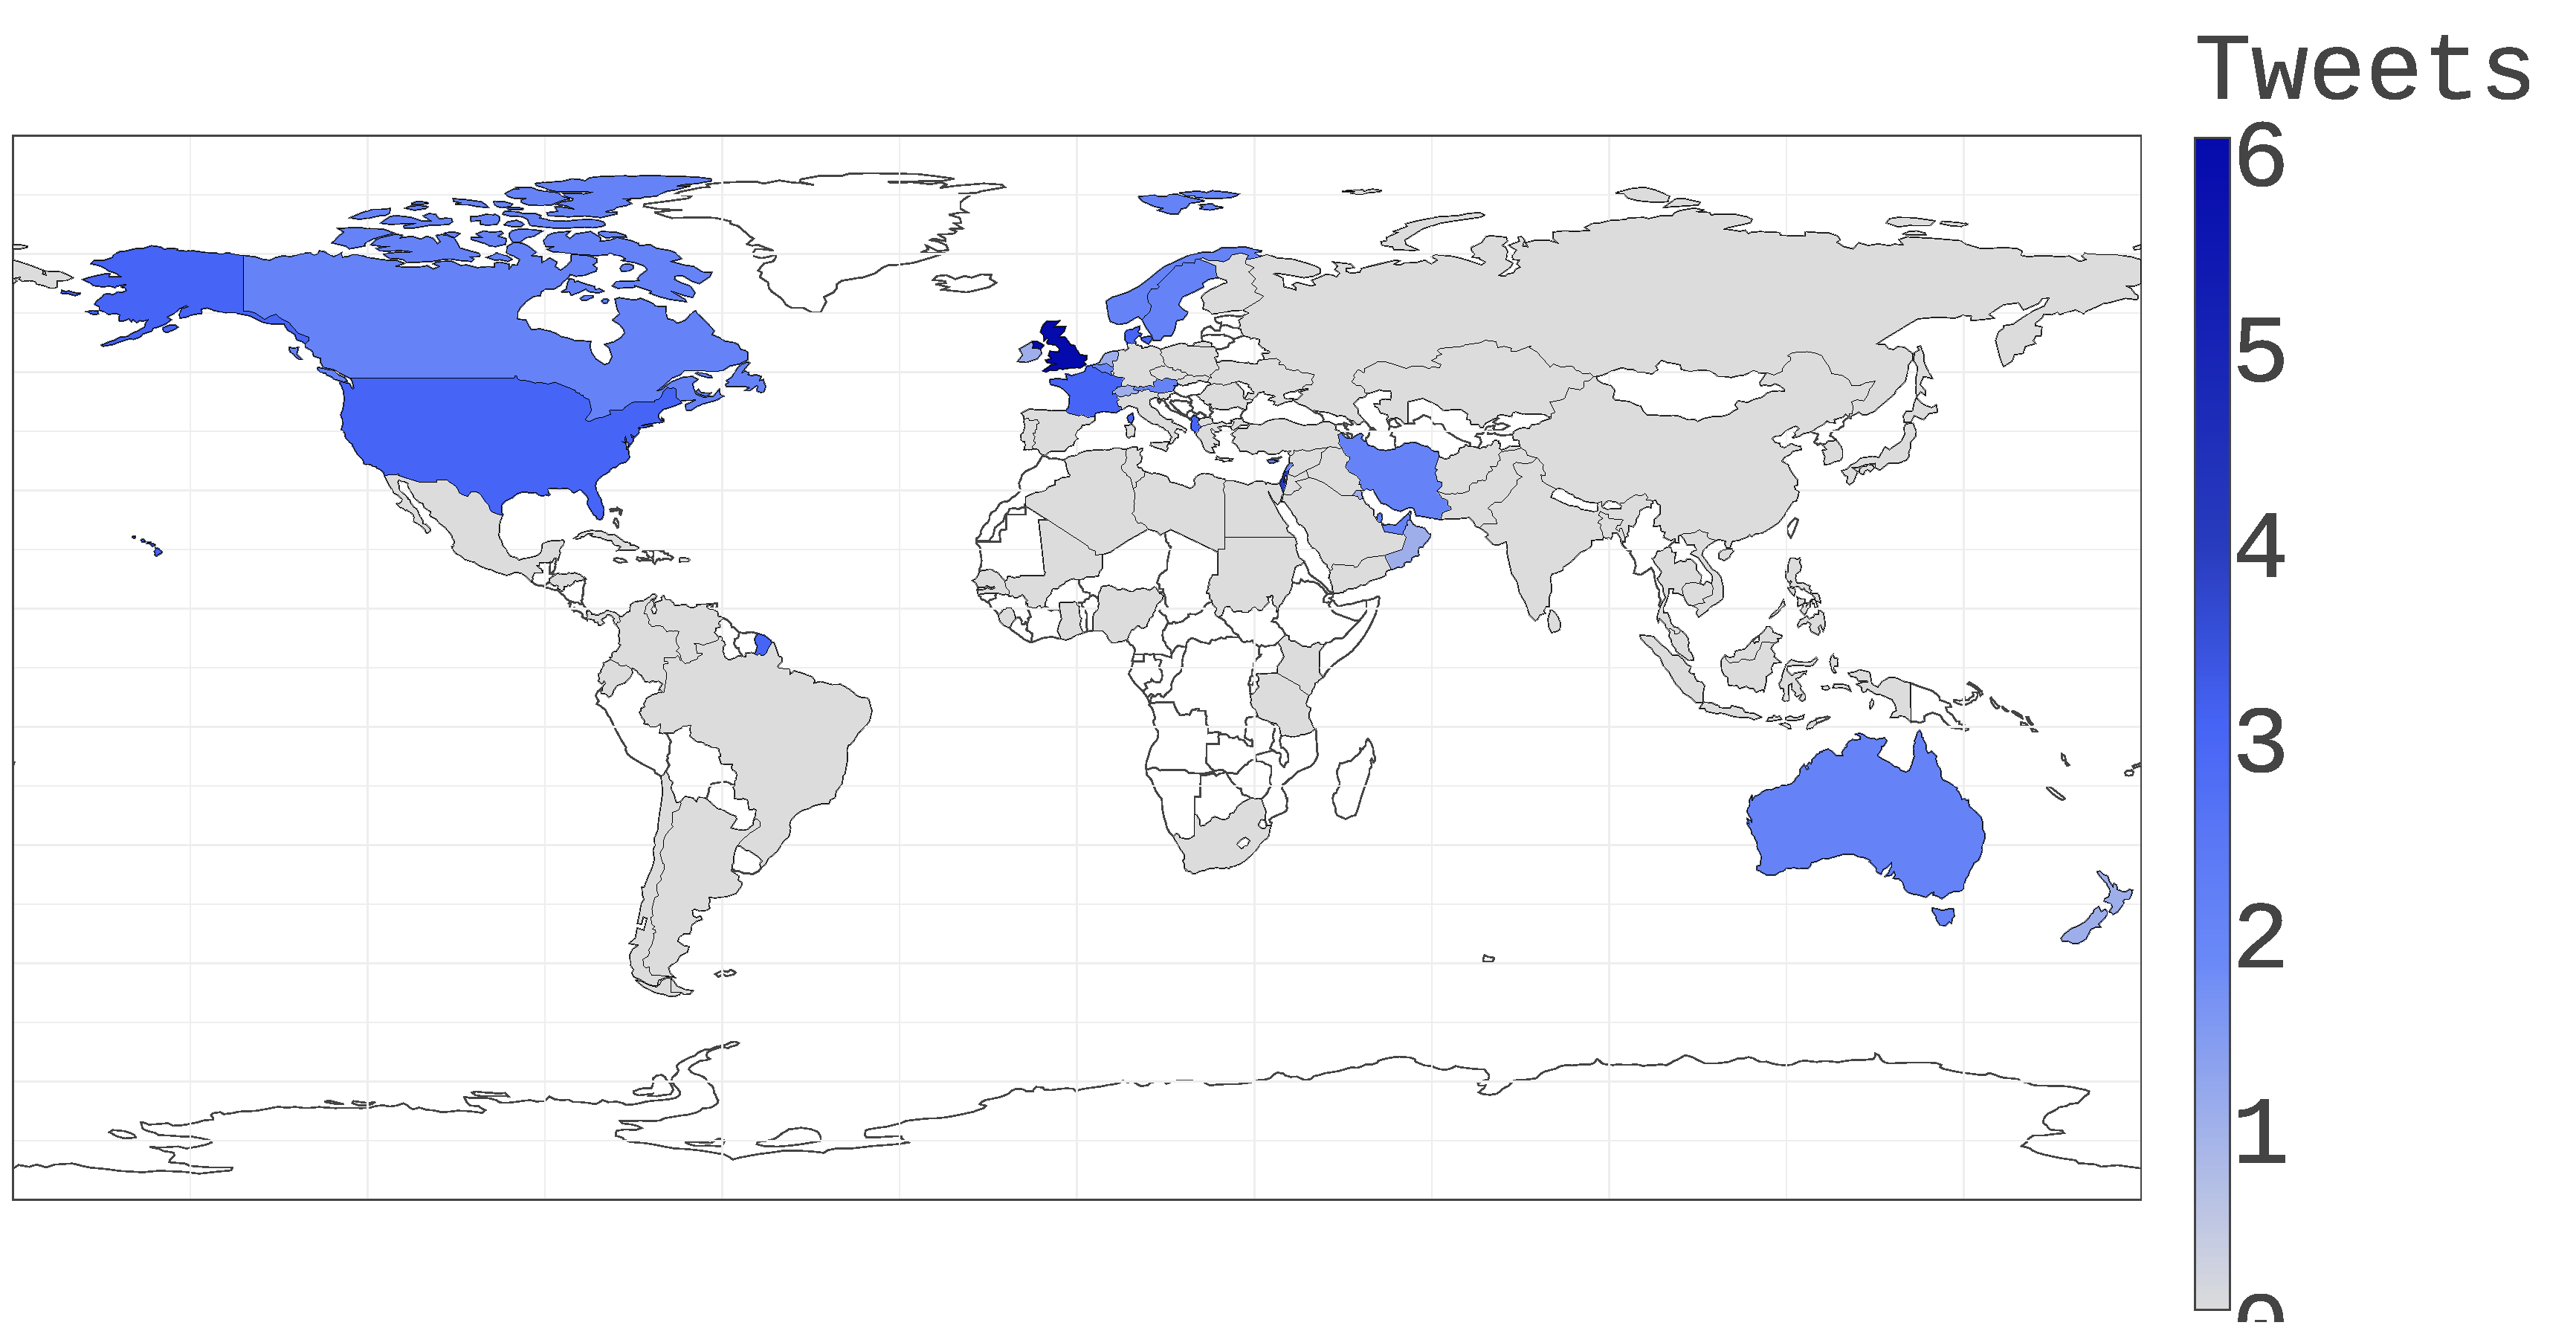
\includegraphics[width=5.3cm]{images/location/world/socialsensor-world-irannucleardeal_location.eps}}
\subfloat[Fig:][Soccer]{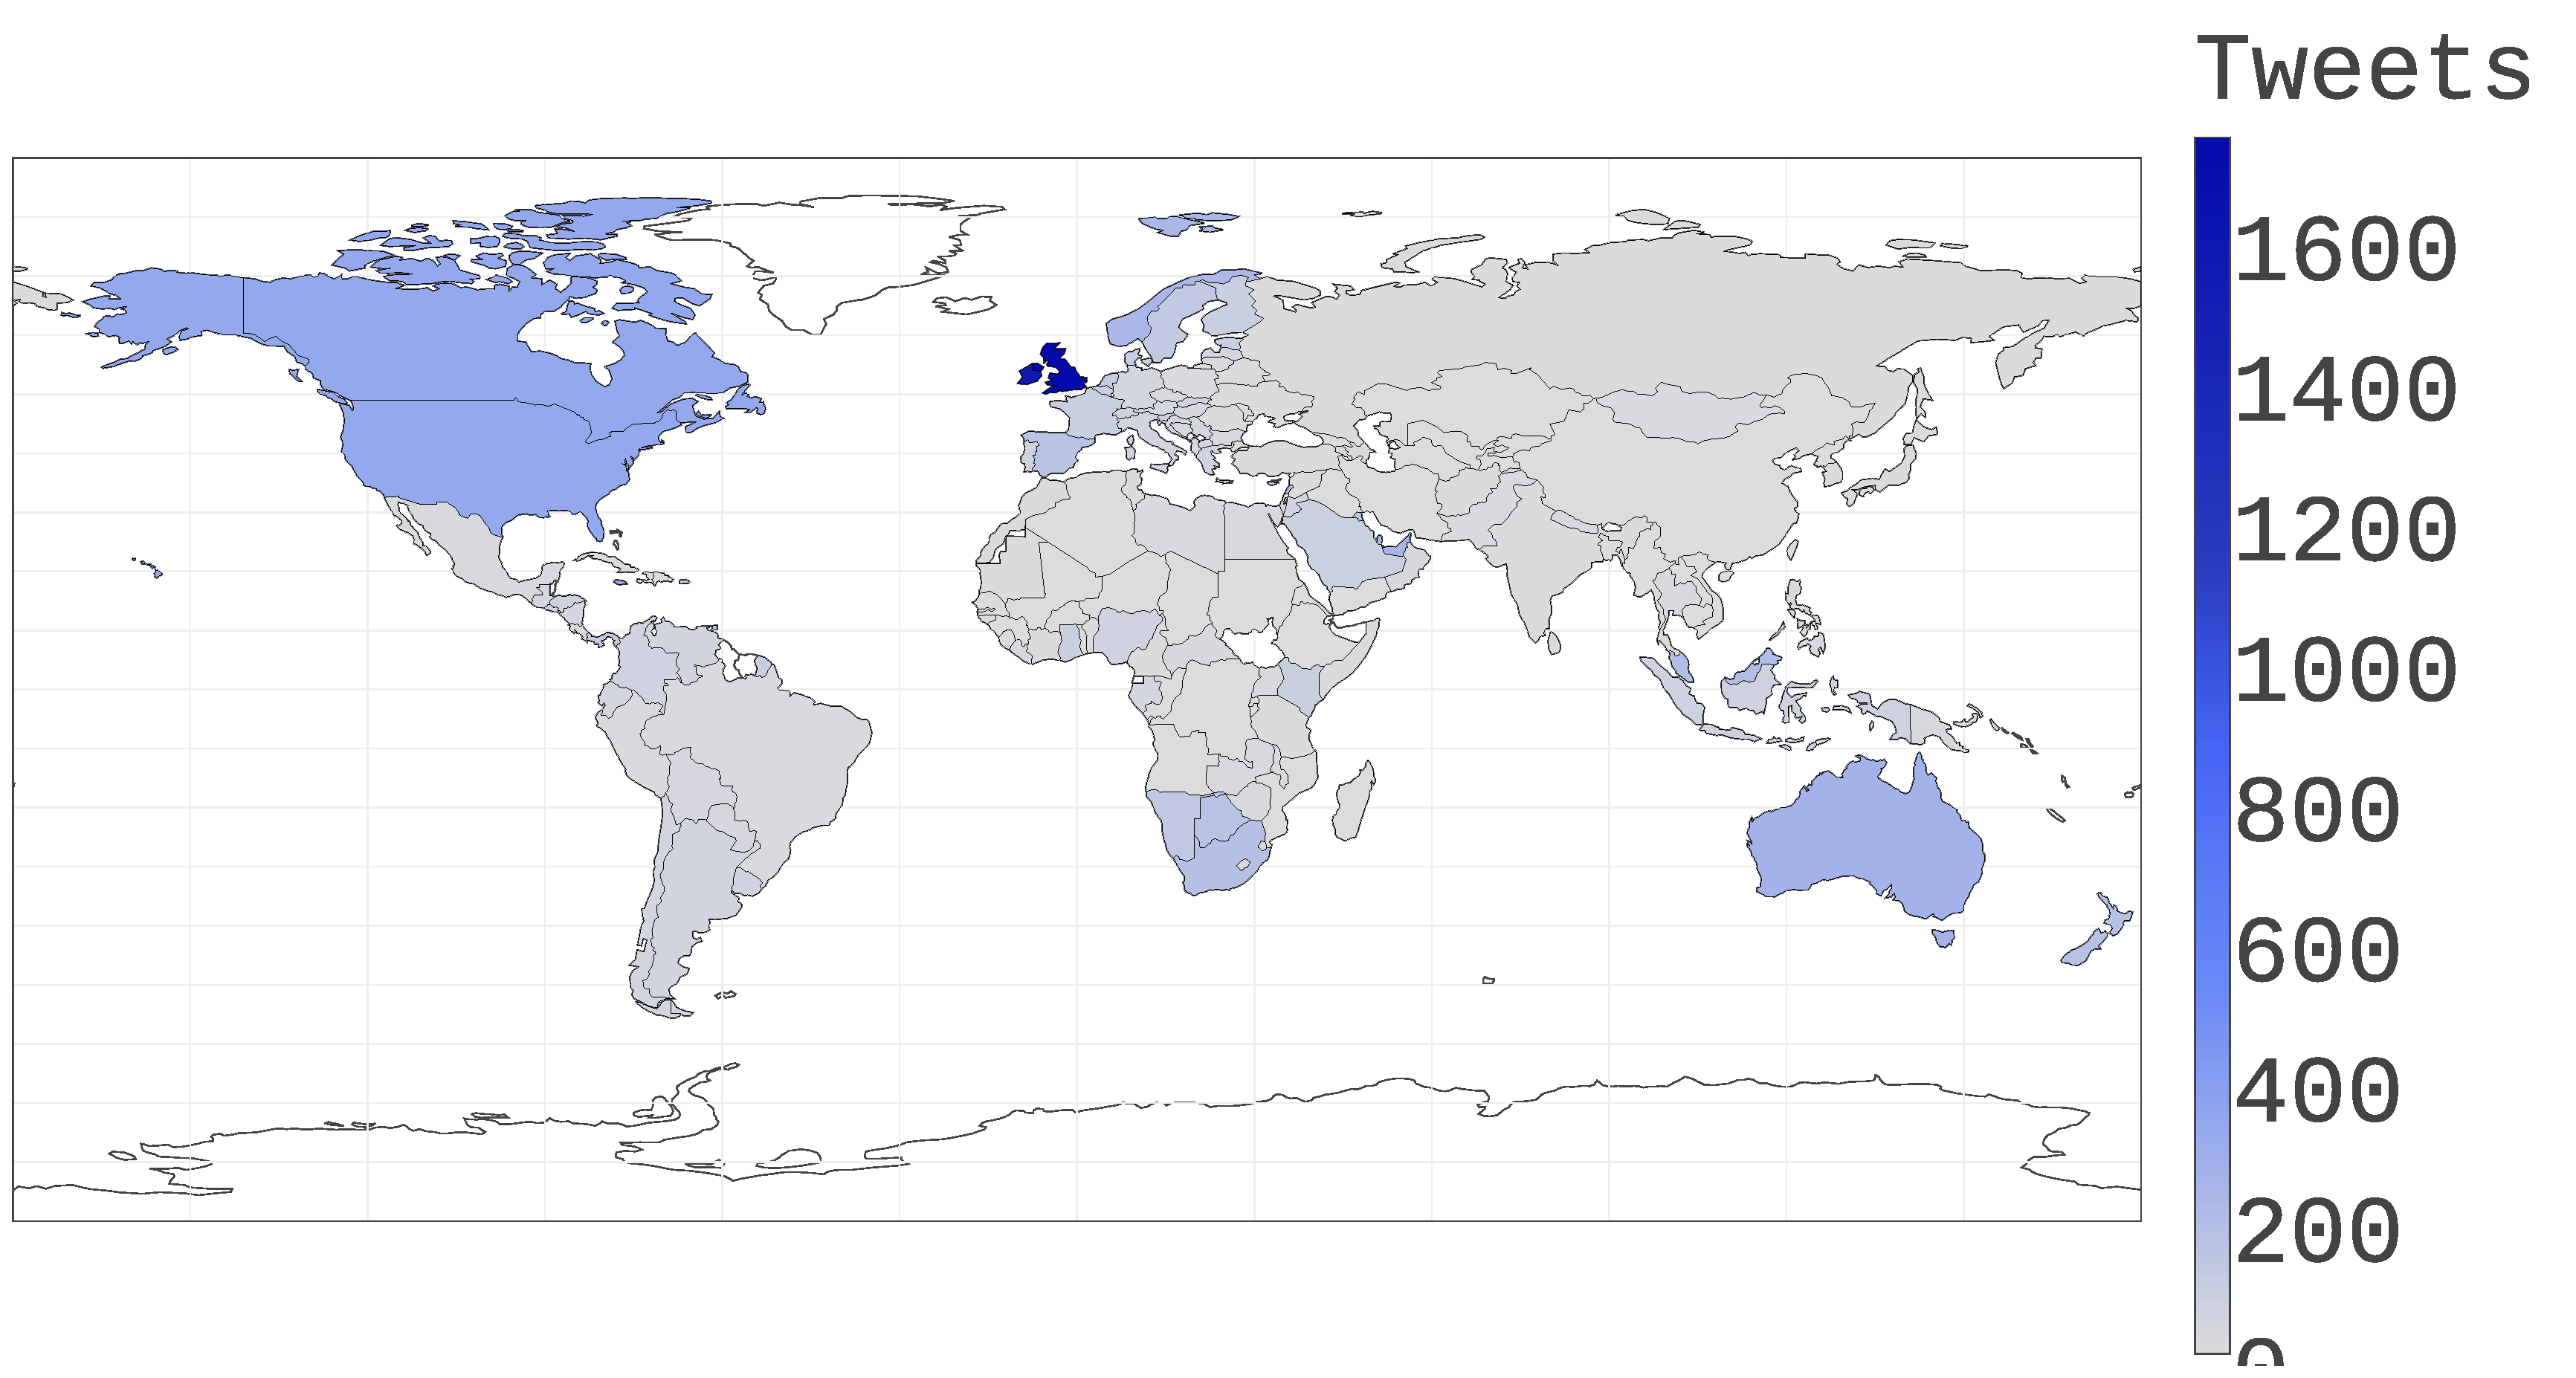
\includegraphics[width=5.3cm]{images/location/world/socialsensor-world-soccer_location.eps}} \\
%\vspace{-10mm}
\subfloat[Fig:][Health Epidemics]{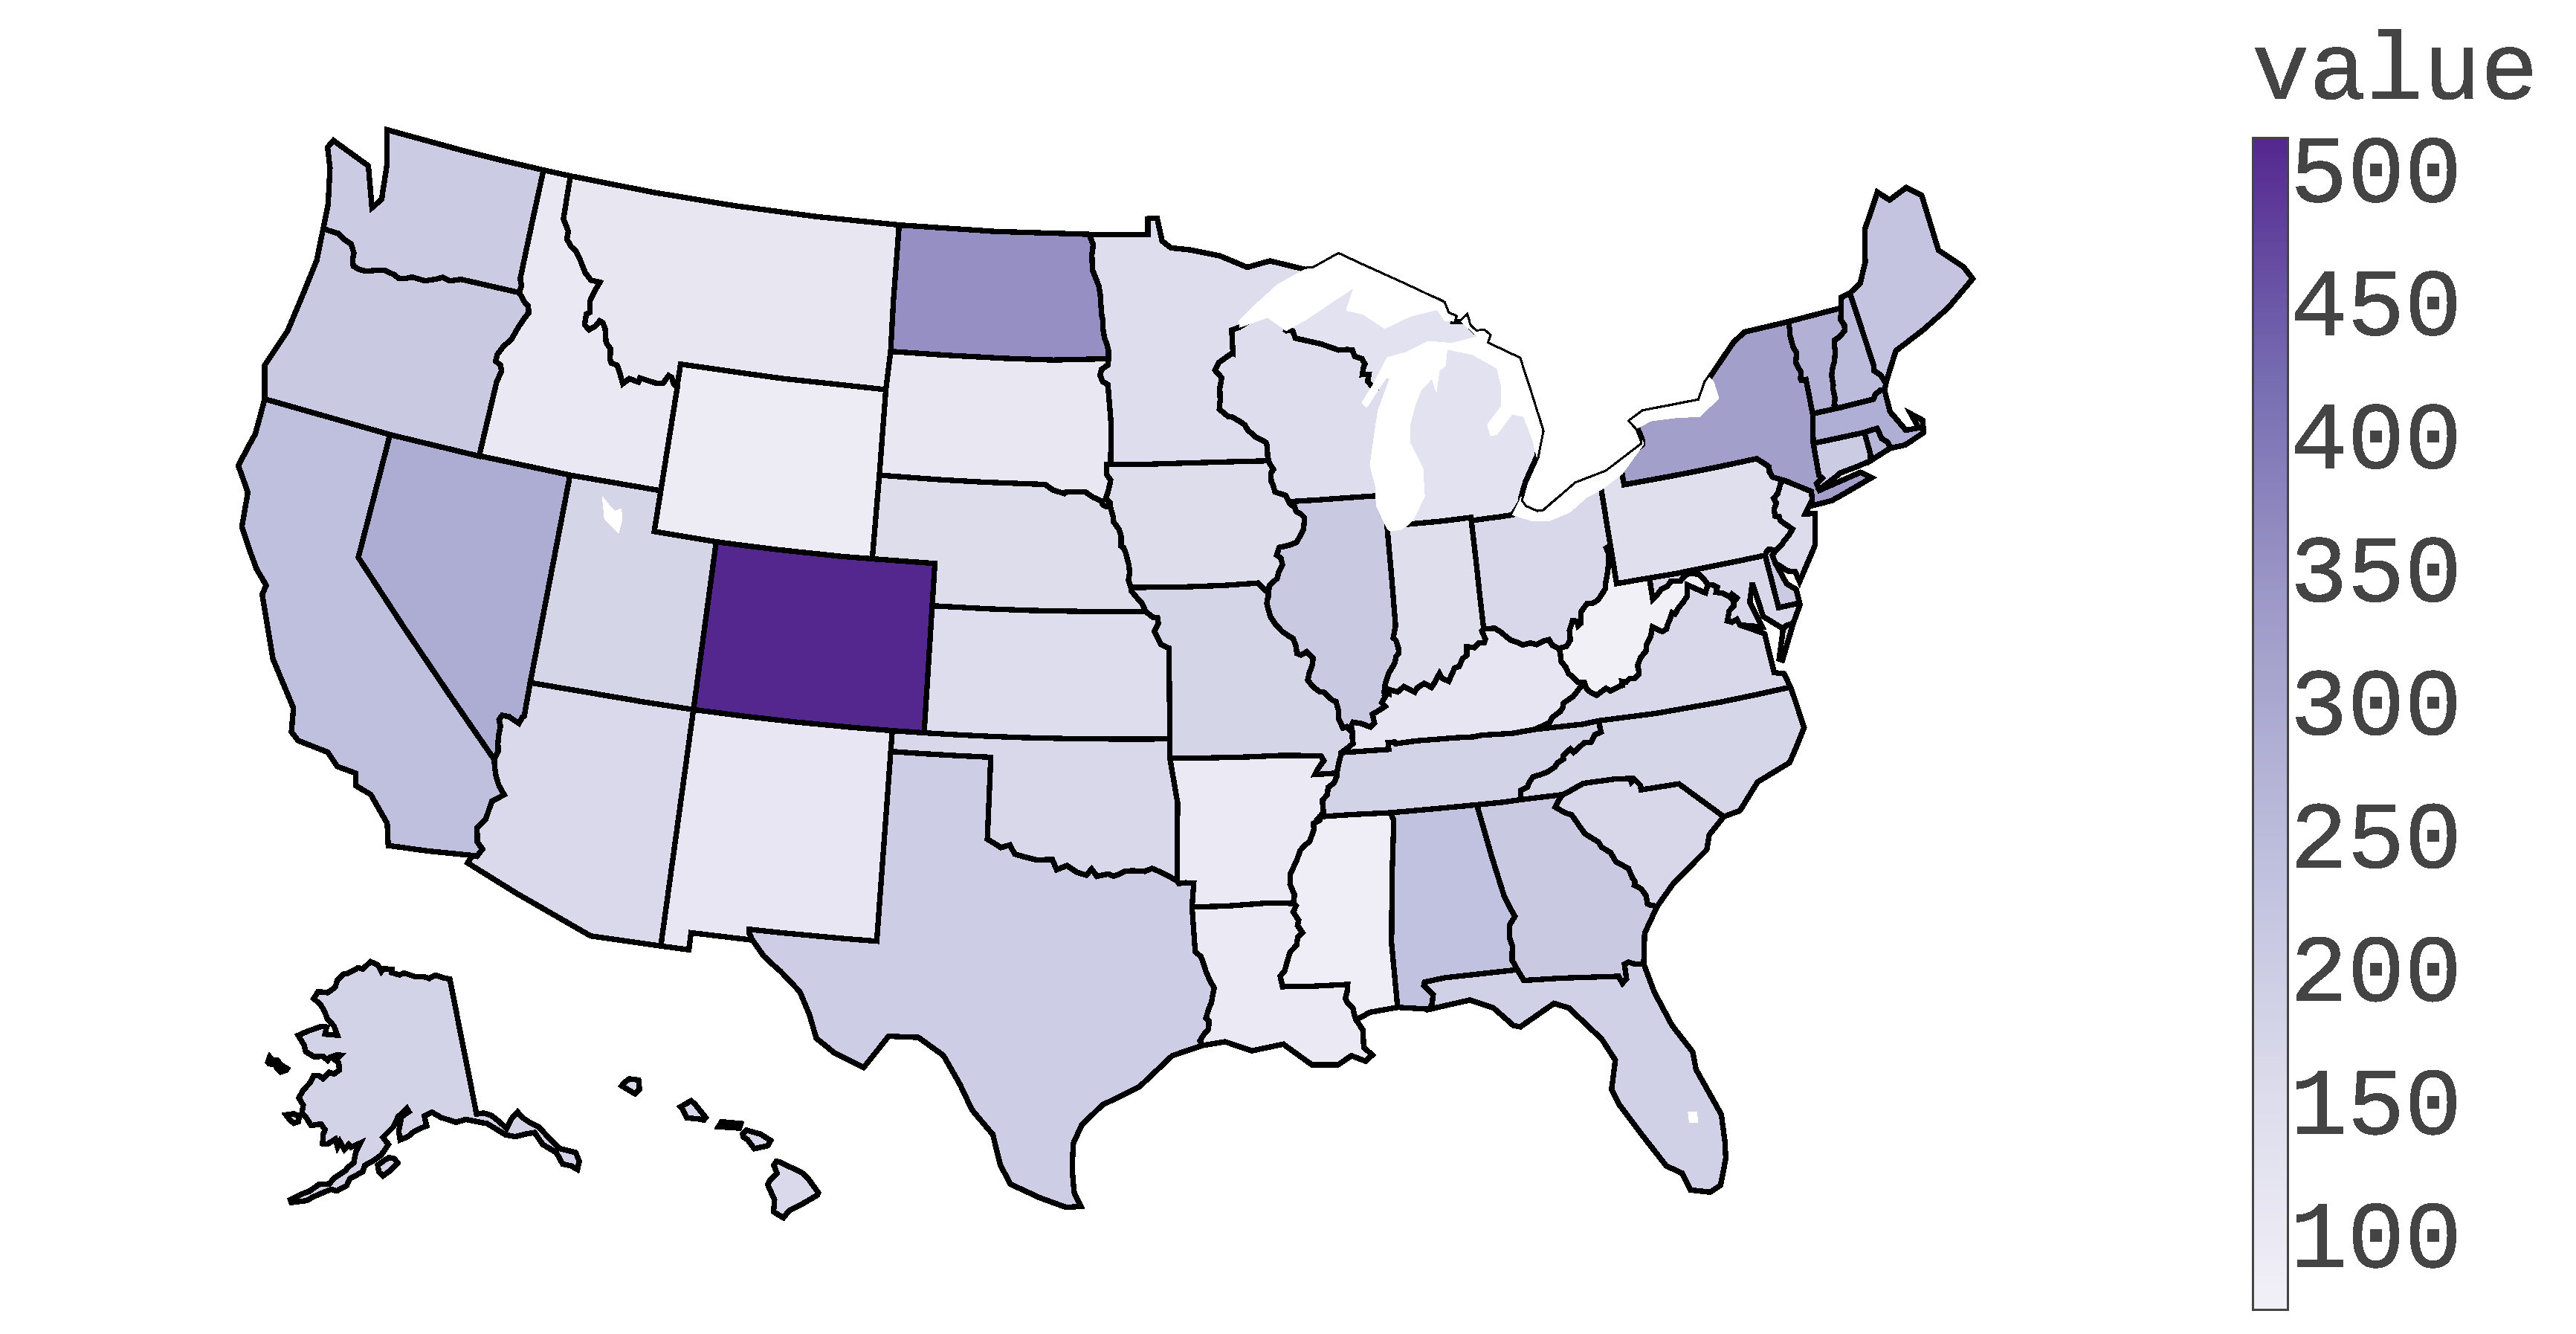
\includegraphics[width=5.3cm]{images/location/states/SocialSensor-us-states-health_epidemics_location.eps}}
\subfloat[Fig:][Social Issues]{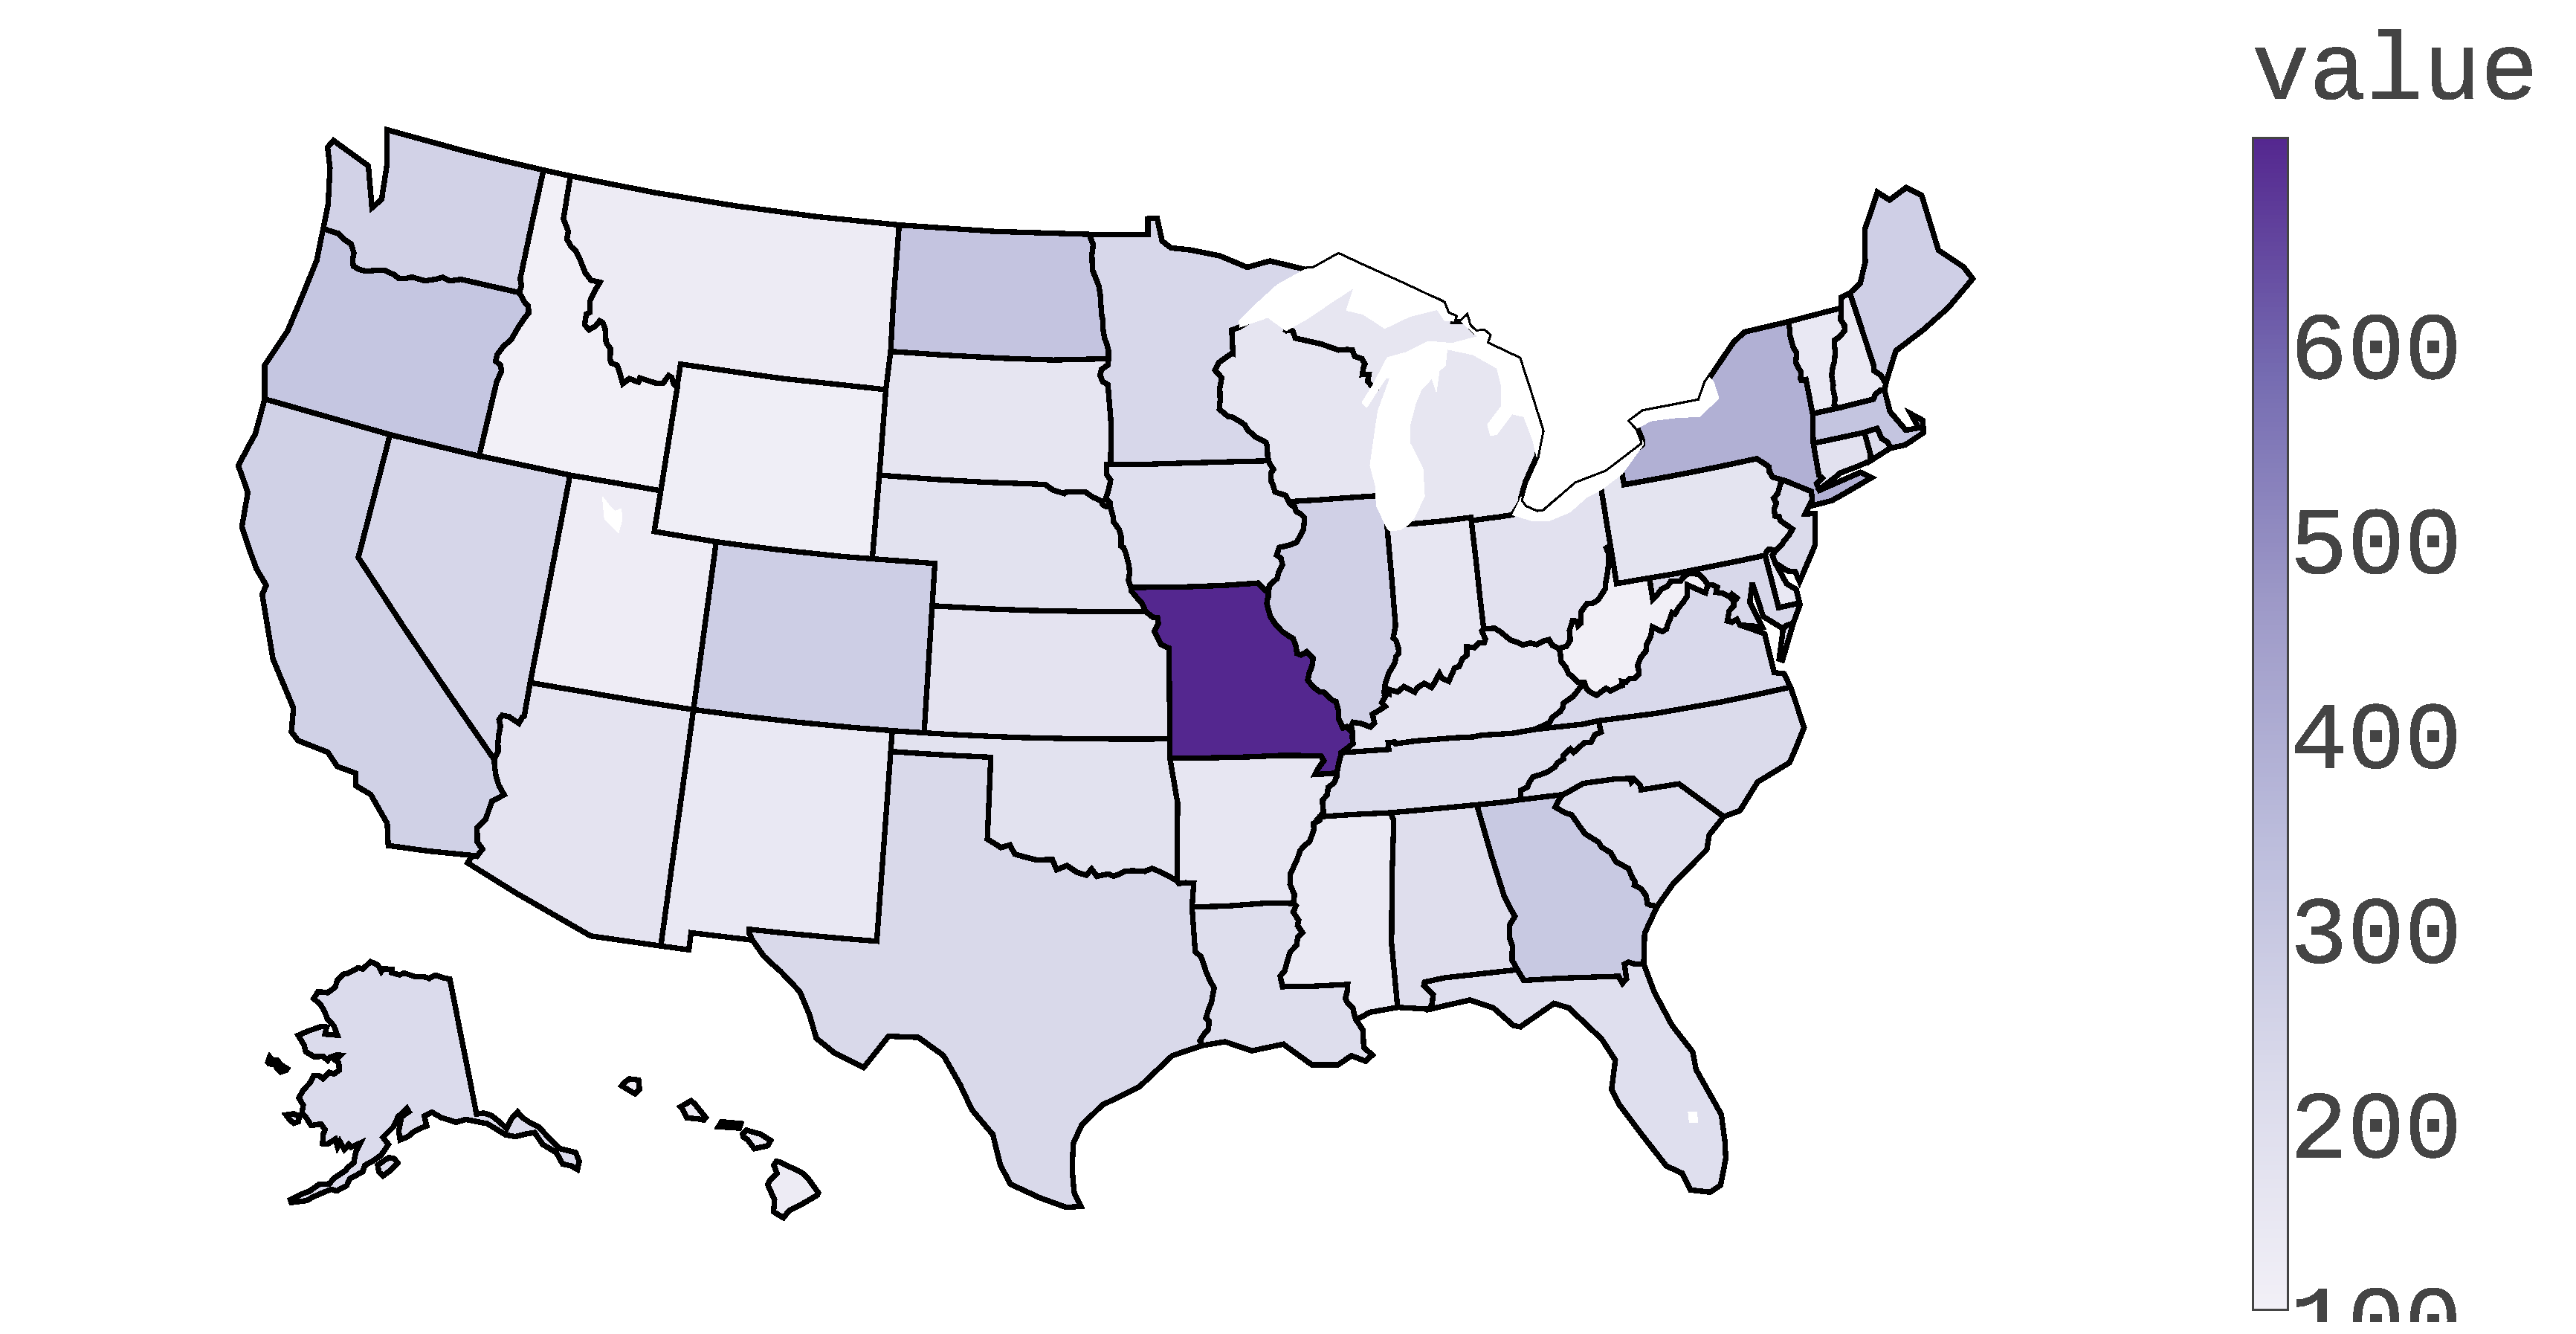
\includegraphics[width=5.3cm]{images/location/states/SocialSensor-us-states-socialissues_location.eps}}
\subfloat[Fig:][Space]{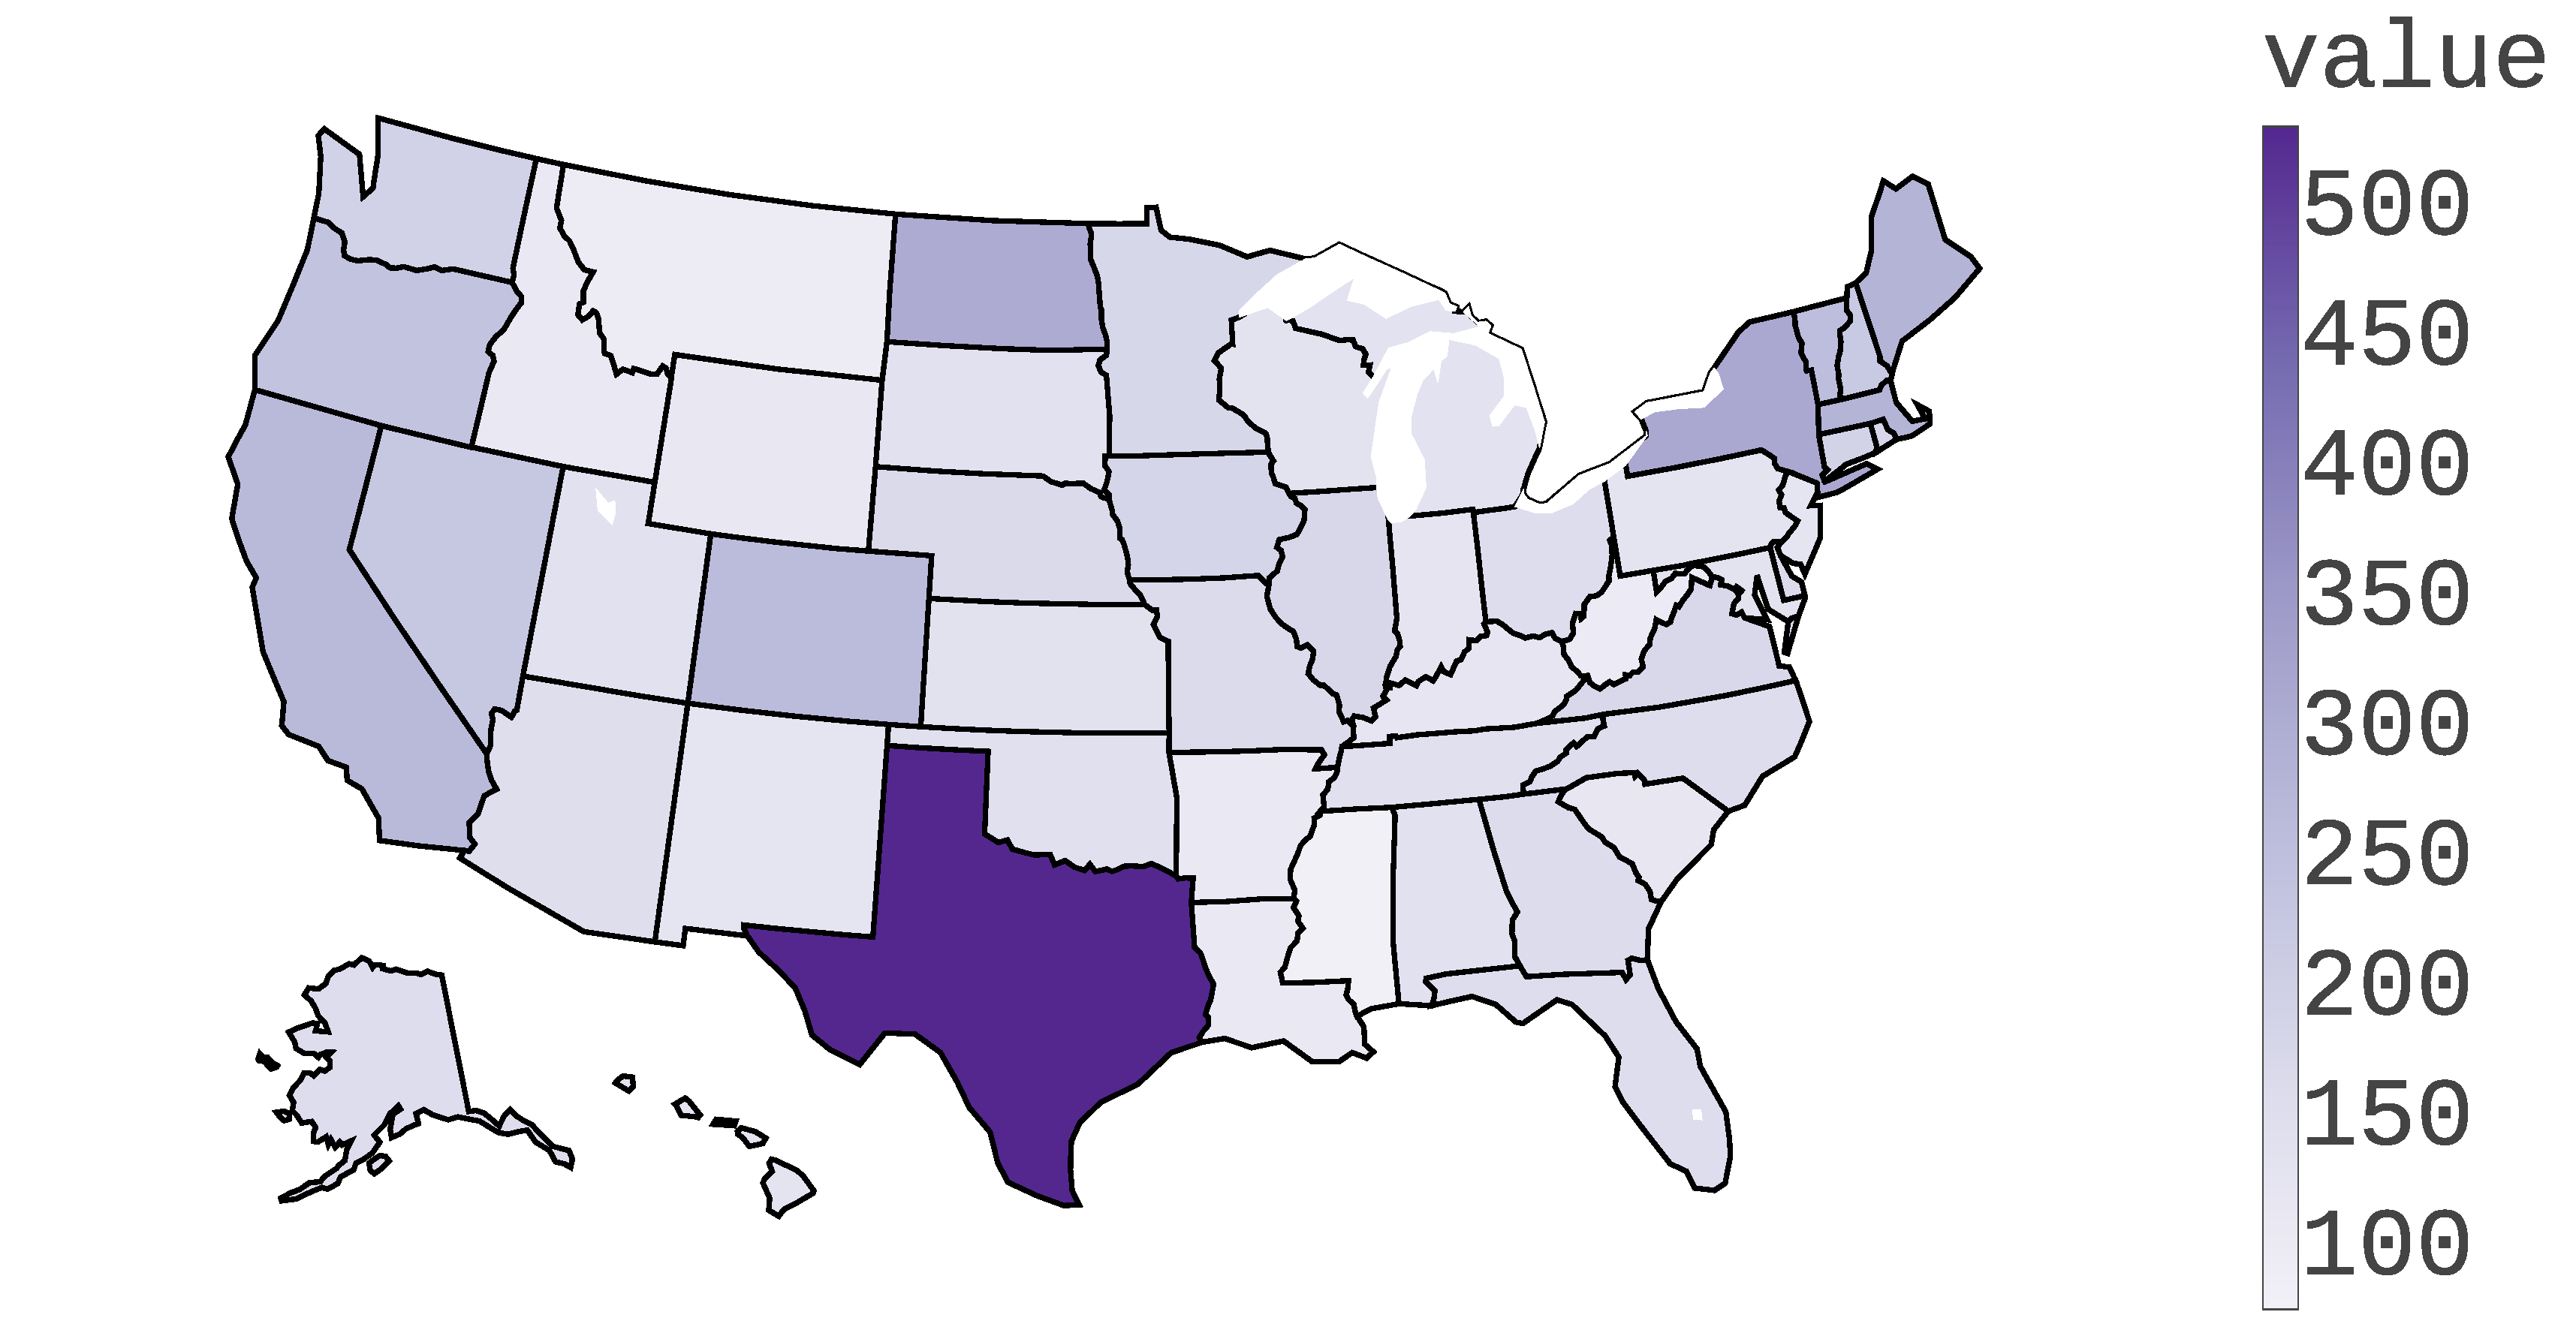
\includegraphics[width=5.3cm]{images/location/states/SocialSensor-us-states-space_location}} \\
\end{tabular}
\end{tabular}
\vspace{-2mm}
\caption {Distribution of tweets across International locations (top row) and U.S. locations (bottom row)}
\label{fig:choropleths}
\end{figure*}
%%%%%%%%%%%%%%%%%%%%%%%%%%%%%%%%%%%%%%%%%%%%%%%%%%%%%%%%%%%%%%%%%%%%%%%%%%%

Now we provide details of the Twitter testbed for topical social sensor learning
that we evaluate in this paper.  We crawled Twitter data using Twitter
Streaming API for two years spanning 2013 and 2014 years.
%This type of crawling provides us with a very sparse set of data, roughly $1\%$ of all tweets \footnote{\hyperref[]{http://allthingsd.com/20101110/twitter-firehose-too-intense-take-a-sip-from-the-garden-hose-or-sample-the-spritzer|}}. 
The total number of tweets collected is $829,026,458$. In the context
of Twitter, we consider five feature types for each tweet.  Each
tweet has a \textit{From} feature (i.e., the person who tweeted it), a
possible \textit{Location} (i.e., a string provided as meta-data), and
a time stamp when it was posted.  A tweet can also contain one or more
of the following:
\begin{itemize}
%NOTE: $$ is not for italics... it is for math mode and has larger math mode spacing
%since adjacent letters are implicitly multiplied.  Use \textit -SPS
\item \textit{Hashtag}: a topical keyword specified using the \# sign.
\item \textit{Mention}: a Twitter username reference using the @ sign. % reply?
\item \textit{Term}:    any non-hashtag and non-mention unigrams. %These uni-grams are later cleaned to remove $Term$s with no meaning (total number of $Term$s before cleaning was $20,234,729$)
\end{itemize}
We provide more detailed statistics about each feature in
Table~\ref{table:featureStatistics}.  For example,
authors (\textit{From} users) have used a median value of $2$
unique hashtags % not average, median!!! -SPS
and a hashtag has been used on average by $10.08$ unique users.

Fig.~\ref{fig:choropleths} shows per capita tweet frequency across
different international and U.S. locations for different topics.
While English speaking countries dominate English tweets, we
see that the Middle East and Malaysia additionally stand out for the
topic of Human Caused Disaster (MH370 incident), Iran and Europe
for the ``Iran deal'', and
soccer for many countries where it is popular.  For U.S. states,
we see that Colorado stands out for health epidemics (both whooping
cough and pneumonic plague), Missouri stands out for social issues
(\#blacklivesmatter in St. Louis), and Texas stands out for space due to
NASA's presence there.

%%%%%%%%%%%%%%%%%%%%%%%%%%%%%%%%%%%%%%%%%%%%%%%%%%%%%%%%%%%%%%%%%%
\begin{table}[t!]
\centering
{\renewcommand{\arraystretch}{1.2}
\resizebox{0.5\textwidth}{!}{%
\begin{tabular}{|c|c|c|c|c|}
%\hline
\multicolumn{5}{c}{\textbf{\#Unique Features}} \\ \hline
\textbf{From} & \textbf{Hashtag} & \textbf{Mention} & \textbf{Location} & \textbf{Term} \\ \hline
95,547,198 & 11,183,410 & 411,341,569 & 58,601 & 20,234,728 \\ \hline %14,197,509
\end{tabular}
}}
%\vspace{.5mm}
%\caption{Number of unique features for each type.}%values for each feature of $829,026,458$ tweets in our Twitter dataset}
%\label{table:featureUnique}
%\end{table}
%
%\begin{table}[t!]
%\centering
{\renewcommand{\arraystretch}{1.2}
\resizebox{0.5\textwidth}{!}{%
\begin{tabular}{|l|c|c|c|c|}
%\hline
\multicolumn{5}{c}{\textbf{Feature Usage in \#Tweets}} \\ \hline
\textbf{Feature} & \textbf{Max} & \textbf{Avg} & \textbf{Median} & \textbf{Max entity} \\ \hline
\textbf{From} & 10,196 & 8.67 & 2 & running\_status \\ \hline
\textbf{Hashtag} & 1,653,159 & 13.91 & 1 & \#retweet \\ \hline
\textbf{Mention} & 6,291 & 1.26 & 1 & null \\ \hline
\textbf{Location} & 10,848,224 & 9,562.34 & 130 & london \\ \hline
\textbf{Term} & 241,896,559 & 492.37 & 1 & rt \\ \hline 
\multicolumn{5}{c}{\textbf{Feature Usage by \#Users}} \\ \hline
\textbf{Hashtag} & 592,363 & 10.08 & 1 & \#retweet \\ \hline
\textbf{Mention} & 26,293 & 5.44 & 1 & dimensionist \\ \hline
\textbf{Location} & 739,120 & 641.5 & 2 & london \\ \hline
\textbf{Term} & 1,799,385 & 6,616.65 & 1 & rt \\ \hline %SHOULD BE FIXED
\multicolumn{5}{c}{\textbf{Feature Using \#Hashtags}} \\ \hline
\textbf{From} & 18,167 & 2 & 0 & daily\_astrodata \\ \hline
\end{tabular}
}}
\caption{Feature Statistics of our $829,026,458$ tweet corpus.} % in our Twitter dataset}
\label{table:featureStatistics}
\end{table}
%%%%%%%%%%%%%%%%%%%%%%%%%%%%%%%%%%%%%%%%%%%%%%%%%%%%%%%%%%%%%%%%%%


\section{Empirical Evaluation}
\label{sec:methodology}
%!TEX root = icwsm2017.tex

%%%%%%%%%%%%%%%%%%%%%%%%%%%%%%%%%%%%%%%%%%%%%%%%%%%%%%%%%%%%%%%%%%
\begin{table*}[t!]
\centering
{\renewcommand{\arraystretch}{1.2}
\resizebox{\textwidth}{!}{%
\begin{tabular}{|l|l|l|l|l|l|l|l|l|l|l|}
\hline
\multicolumn{1}{|c|}{}                    & \multicolumn{1}{c|}{\textbf{Tennis}} & \multicolumn{1}{c|}{\textbf{Space}} & \multicolumn{1}{c|}{\textbf{Soccer}} & \multicolumn{1}{c|}{\textbf{IranDeal}} & \multicolumn{1}{c|}{\textbf{HumanDisaster}} & \multicolumn{1}{c|}{\textbf{CelebrityDeath}} & \multicolumn{1}{c|}{\textbf{SocialIssues}} & \multicolumn{1}{c|}{\textbf{NaturalDisaster}} & \multicolumn{1}{c|}{\textbf{Epidemics}} & \multicolumn{1}{c|}{\textbf{LGBT}} \\ \hline
\textbf{\#TrainHashtags}                  & \multicolumn{1}{c|}{58}              & \multicolumn{1}{c|}{98}             & \multicolumn{1}{c|}{126}             & \multicolumn{1}{c|}{12}                & \multicolumn{1}{c|}{49}                     & \multicolumn{1}{c|}{28}                      & \multicolumn{1}{c|}{31}                    & \multicolumn{1}{c|}{31}                       & \multicolumn{1}{c|}{52}                 & \multicolumn{1}{c|}{29}            \\ \hline
\textbf{\#TestHashtags}                   & \multicolumn{1}{c|}{36}              & \multicolumn{1}{c|}{63}             & \multicolumn{1}{c|}{81}              & \multicolumn{1}{c|}{5}                 & \multicolumn{1}{c|}{29}                     & \multicolumn{1}{c|}{16}                      & \multicolumn{1}{c|}{19}                    & \multicolumn{1}{c|}{19}                       & \multicolumn{1}{c|}{33}                 & \multicolumn{1}{c|}{17}            \\ \hline
\textbf{\#TopicalTweets}                  & \multicolumn{1}{c|}{55,053}          & \multicolumn{1}{c|}{239,719}        & \multicolumn{1}{c|}{860,389}         & \multicolumn{1}{c|}{8,762}             & \multicolumn{1}{c|}{408,304}                & \multicolumn{1}{c|}{163,890}                 & \multicolumn{1}{c|}{230,058}               & \multicolumn{1}{c|}{230,058}                  & \multicolumn{1}{c|}{210,217}            & \multicolumn{1}{c|}{282,527}       \\ \hline
\multirow{5}{*}{\textbf{Sample Hashtags}} & \#usopenchampion                     & \#asteroids                         & \#worldcup                           & \#irandeal                             & {\footnotesize \#gazaunderattack}                           & \#robinwilliams                              & \#policebrutality                          & \#earthquake                             & \#ebola                                 & \#loveislove                       \\ \cline{2-11} 
                                          & \#novakdjokovic                      & \#astronauts                        & \#lovesoccer                         & \#iranfreedom                          & {\footnotesize \#childrenofsyria}                           & \#ripmandela                                 & \#michaelbrown                             & \#storm                                & \#virus                                 & \#gaypride                         \\ \cline{2-11} 
                                          & \#wimbledon                          & \#satellite                         & \#fifa                               & \#irantalk                             & \#iraqwar                                   & \#ripjoanrivers                              & \#justice4all                              & \#tsunami                                 & \#vaccine                               & \#uniteblue                        \\ \cline{2-11} 
                                          & \#womenstennis                       & \#spacecraft                        & \#realmadrid                         & \#rouhani                              & \#bombthreat                                & \#mandela                                    & \#freetheweed                              & \#abfloods                                 & \#chickenpox                            & \#homo                             \\ \cline{2-11} 
                                          & \#tennisnews                         & \#telescope                         & \#beckham                            & \#nuclearpower                         & \#isis                                      & \#paulwalker                                 & \#newnjgunlaw                              & \#hurricanekatrina                                 & \#theplague                             & {\footnotesize \#gaymarriage}                      \\ \hline
\end{tabular}
}
}
\caption{Test/Train Hashtag samples and statistics.}
\label{table:sampleHashtags}
\end{table*}
%%%%%%%%%%%%%%%%%%%%%%%%%%%%%%%%%%%%%%%%%%%%%%%%%%%%%%%%%%%%%%%%%%


%%%%%%%%%%%%%%%%%%%%%%%%%%%%%%%%%%%%%%%%%%%%%%%%%%%%%%%%%%%%%%%%%%
\begin{table}[t!]
\vspace{-0.5mm}
\centering
{\footnotesize
%\small
\renewcommand{\arraystretch}{1.2}
\begin{tabular}{|l|c|c|}
\hline
 & \textbf{Threshold} & \textbf{\#Unique Values} \\ \hline
\textbf{From} & 159 & 361,789 \\ \hline
\textbf{Hashtag} & 159 & 184,702 \\ \hline
\textbf{Mention} & 159 & 244,478 \\ \hline
\textbf{Location} & 50 & 57,767 \\ \hline
\textbf{Term} & 50 & 317,846 \\ \hline
\textbf{Features (CF)} & - & 1,166,582 \\ \hline
\end{tabular}
}
\vspace{-1mm}
\caption{Cutoff threshold and corresponding number of unique values of candidate features \textit{CF} for learning.}
\label{table:learningFeatures}
\vspace{-1.5mm}
\end{table}
%%%%%%%%%%%%%%%%%%%%%%%%%%%%%%%%%%%%%%%%%%%%%%%%%%%%%%%%%%%%%%%%%%


%%%%%%%%%%%%%%%%%%%%%%%%%%%%%%%%%%%%%%%%%%%%%%%%%%%%%%%%%%%%%%%%%%
\begin{table*}[t!]
\centering
{\renewcommand{\arraystretch}{1.2}
\resizebox{\textwidth}{!}{%
\begin{tabular}{|l|l|l|l|l|l|l|l|l|l|l|l|l|}
\hline
 &  & \textbf{Tennis} & \textbf{Space} & \textbf{Soccer} & \textbf{IranDeal} & \textbf{HumanDisaster} & \textbf{CelebrityDeath} & \textbf{SocialIssues} & \textbf{NaturalDisaster} & \textbf{Epidemics} & \textbf{LGBT} & \textbf{Mean} \\ \hline
\textbf{LR} & \textbf{AP} & \textbf{0.918} & 0.870 & 0.827 & 0.811 & 0.761 & 0.719 & 0.498 & \textbf{0.338} & \textbf{0.329} & \textbf{0.165} & \textbf{0.623$\pm$0.19} \\ \hline
\textbf{NB} & \textbf{AP} & 0.908 & \textbf{0.897} & 0.731 & \textbf{0.824} & \textbf{0.785} & \textbf{0.748} & \textbf{0.623} & 0.267 & 0.178 & 0.092 & 0.605$\pm$0.22 \\ \hline
\textbf{Rocchio} & \textbf{AP} & 0.690 & 0.221 & \textbf{0.899} & 0.584 & 0.481 & 0.253 & 0.393 & 0.210 & 0.255 & 0.089 & 0.407$\pm$0.18 \\ \hline
\textbf{RankSVM} & \textbf{AP} & 0.702 & 0.840 & 0.674 & 0.586 & 0.603 & 0.469 & 0.370 & 0.248 & 0.136 & 0.082 & 0.471$\pm$0.18 \\ \hline \hline
\textbf{LR} & \textbf{P@10} & \textbf{1.000} & 0.000 & 0.200 & 0.700 & \textbf{0.600} & 0.000 & 0.100 & 0.200 & 0.300 & \textbf{0.500} & 0.360$\pm$0.24 \\ \hline
\textbf{NB} & \textbf{P@10} & \textbf{1.000} & \textbf{0.900} & 0.700 & 0.600 & \textbf{0.600} & \textbf{0.700} & \textbf{1.000} & 0.100 & 0.400 & 0.100 & \textbf{0.610$\pm$0.23} \\ \hline
\textbf{Rocchio} & \textbf{P@10} & 0.800 & 0.000 & \textbf{1.000} & \textbf{0.900} & 0.000 & 0.000 & 0.000 & \textbf{0.500} & \textbf{0.500} & 0.100 & 0.380$\pm$0.29 \\ \hline
\textbf{RankSVM} & \textbf{P@10} & \textbf{1.000} & 0.800 & 0.600 & 0.800 & 0.400 & 0.300 & 0.000 & 0.100 & 0.000 & 0.200 & 0.420$\pm$0.26 \\ \hline \hline
\textbf{LR} & \textbf{P@100} & 0.950 & 0.580 & 0.650 & 0.870 & 0.620 & 0.490 & 0.640 & \textbf{0.690} & \textbf{0.790} & \textbf{0.210} & \textbf{0.649$\pm$0.15} \\ \hline
\textbf{NB} & \textbf{P@100} & \textbf{0.980} & \textbf{0.850} & 0.600 & \textbf{0.880} & 0.750 & \textbf{0.860} & \textbf{0.730} & 0.230 & 0.090 & 0.190 & 0.616$\pm$0.23 \\ \hline
\textbf{Rocchio} & \textbf{P@100} & \textbf{0.980} & 0.000 & \textbf{1.000} & 0.690 & 0.170 & 0.000 & 0.280 & 0.170 & 0.680 & 0.120 & 0.409$\pm$0.28 \\ \hline
\textbf{RankSVM} & \textbf{P@100} & 0.730 & 0.720 & 0.310 & 0.700 & \textbf{0.880} & 0.440 & 0.480 & 0.340 & 0.020 & 0.100 & 0.472$\pm$0.20 \\ \hline \hline
\textbf{LR} & \textbf{P@1000} & \textbf{0.963} & \textbf{0.954} & 0.816 & \textbf{0.218} & 0.899 & 0.833 & \textbf{0.215} & 0.192 & \textbf{0.343} & \textbf{0.071} & \textbf{0.550$\pm$0.26} \\ \hline
\textbf{NB} & \textbf{P@1000} & 0.954 & \textbf{0.954} & 0.716 & \textbf{0.218} & \textbf{0.904} & \textbf{0.881} & \textbf{0.215} & \textbf{0.195} & 0.141 & 0.060 & 0.524$\pm$0.28 \\ \hline
\textbf{Rocchio} & \textbf{P@1000} & 0.604 & 0.000 & \textbf{0.925} & \textbf{0.218} & 0.359 & 0.000 & \textbf{0.215} & 0.167 & 0.144 & 0.065 & 0.270$\pm$0.21 \\ \hline
\textbf{RankSVM} & \textbf{P@1000} & 0.799 & 0.922 & 0.764 & \textbf{0.218} & 0.525 & 0.547 & \textbf{0.215} & 0.173 & 0.154 & 0.064 & 0.438$\pm$0.22 \\ \hline
\end{tabular}
}}
\caption{Performance of topical classifier learning algorithms across metrics and topics with the
mean performance over all topics shown in the right column. The best performance per metric is shown in bold.} 
\label{table:results2}
\end{table*}
%%%%%%%%%%%%%%%%%%%%%%%%%%%%%%%%%%%%%%%%%%%%%%%%%%%%%%%%%%%%%%%%%%

%How we curated hashtags: need to make up good story here.  Inner-annotator agreement of 3/4.
With the formal definition of learning topical classifiers provided
in Sec.~\ref{sec:lss} and the overview of our data in
Sec.~\ref{sec:datasetStatistics}, we proceed to outline our
experimental methodology on our Twitter corpus.  We manually curated a
broad thematic range of 10 topics shown in the top row of
Table~\ref{table:sampleHashtags}
%\begin{align*}
%T = \{ & \textit{Tennis}, \textit{Space}, \textit{Soccer}, \textit{IranDeal}, \textit{HumanDisaster}, \\
%       & \textit{CelebrityDeath}, \textit{SocialIssues}, \textit{NaturalDisaster}, \\
%       & \textit{Epidemics}, \textit{LGBT} \} 
%\end{align*}
by annotating hashtag sets $H^t$ for each topic $t \in T$.  We used 4
independent annotators to query the Twitter search API to identify
candidate hashtags for each topic, requiring an inner-annotator
agreement of 3 annotators to permit a hashtag to be assigned to a
topic set.  Per topic, hashtags were split into train and test sets
according to their first usage time stamp roughly according to a 3/5
to 2/5 proportion (the test interval spanned between 9-14 months).  
The train set was further temporally subdivided
into train and validation hashtag sets according to a 5/6 to 1/6
proportion.  We show a variety of statistics and five sample hashtags
per topic in Table~\ref{table:sampleHashtags}.  Here we can see that
different topics had varying prevalence in the data
with \textit{Soccer} being the most tweeted topic
and \textit{IranDeal} being the least tweeted according to our curated
hashtags.

As noted in Sec.~\ref{sec:datasetStatistics}, positively occurring
features $D_i^+$ in our $d_i$ may include
\textit{From}, \textit{Mention}, \textit{Location}, \textit{Term}, and \textit{Hashtag} features.
%The summation of number of unique values of features shown in Table.~\ref{table:featureStatistics} results in a total number of $538,365,507$ features. As noted earlier, we are working on a $829,026,458$ tweet corpus. Thus with great number of features and tweets, there is a need for techniques to annotate the data and select a subset of features for learning. 
%
%We explained manual hashtag curation for each topic as a proxy for labeling the tweets. More specifically, the hashtag set $H^{t}$ for each topic $t \in T$ is curated with two annotators individually. Inner-annotator agreement is achieved by reviewing and merging these sets with two more individuals.  provides samples of hashtags, number of train hashtags, test hashtags, and topical tweets for each topic.
Because we have a total of $538,365,507$ unique features in our
Twitter corpus, it is critical to pare this down to a size amenable
for efficient learning and robust to overfitting.  To this end, we
thresholded all features according to the frequencies listed in
Table~\ref{table:learningFeatures}.  The rationale in our thresholding
was initially that all features should have the same frequency cutoff
in order to achieve roughtly 1 million features.  However, in 
initial experimentation, we found that a high threshold pruned a large
number of informative terms and locations.  To this end, we lowered
the threshold for terms and locations noting that even at these
adjusted thresholds, we still have more authors than terms.  We
also removed common English stopwords which further reduced the
unique term count.  Overall, we end up with $1,166,582$
candidate features (\textit{CF}) for learning topical classifiers.

%Regarding feature selection, it is impossible to learn a model on total number of $538,365,507$ features. To learn such a model would require a very large set of training samples, and, feature vectors would be extremely sparse considering $140$ characters limitation of Twitter. Therefore, we performed a primary feature selection based on frequency of each feature by:
%\begin{itemize}
%\item Cleaning the \textit{Term} feature to remove stop-words
%\item Choosing a cut-off threshold on the frequency of features
%\end{itemize} 
%This results in almost $1$ million features. The detailed values of cut-off thresholds and number of remaining unique values for each feature is shown in . Since \textit{Term} and \textit{Location} features exhibited fewer unique values in the corpus, we chose a lower threshold for these features.

%Train/validation/test split date selection -- temporally .5,.1,.4
%\label{label:split}
%In order to conduct our experiments, the train, validation and test set of tweets are formed by temporally dividing the dataset over $2$ years. Since our tweet labeling is through topical hashtags, this division is done in a way to preserve sufficient number of hashtags for train, validation, and test timespan. To this purpose, hashtags are divided based on their birthday with $50$ percent of hashtags born at train timespan, $10$ percent born at validation timespan, and the last $40$ percent born at test timespan.


%Feature selection: threshold per feature 159 and 50 (just explain rationale for lower hashtag and location thresholds).

\subsection{Supervised Learning Algorithms}

With our labeled training and validation datasets defined in
Sec.~\ref{sec:lss} and our candidate feature set \textit{CF} defined
previously, we proceed to apply different probabilistic classification and ranking
algorithms to generate a score function $f^t$ for learning topical classifiers 
as defined in Sec.~\ref{sec:lss}.  In this paper, we experiment with
the following four state-of-the-art supervised classification and ranking methods:
\begin{enumerate}
\item {\bf Logistic Regression} using LibLinear~\cite{liblinear}
\item {\bf Bernoulli Na\"{i}ve Bayes}~\cite{mccallum98nb}
\item {\bf Rocchio}~\cite{manning_ir}\\(a centroid-based classifier)
\item {\bf RankSVM}~\cite{largescale_ranksvm}
\end{enumerate}

As outlined in Sec~\ref{sec:lss}, tuning of hyperparameters on a validation
dataset is critical.  In our experiments, we tune the following hyperparameters:
\begin{itemize}
\item \textit{Logistic Regression}: $L_2$ regularization constant $C$ is tuned for $C \in \{1E-12, 1E-11, ..., 1E+11, 1E+12\}$.
\item \textit{Na\"{i}ve Bayes}: Dirichlet prior $\alpha$ is tuned for $\alpha \in \{1E-20, 1E-15, 1E-8, 1E-3, 1E-1, 1\}$.
\item \textit{All Classfiers}: The number of top features $M$ selected based on their Mutual Information is tuned for $M \in \{1E2, 1E3, 1E4, 1E5, 1166582 \textrm{ (all features) } \}$.
\end{itemize}
We remark that many algorithms such as Naive Bayes and Rocchio
performed better with feature selection and hence we used feature
selection for all algorithms (where it is possible to select all
features).  Hyperparameter tuning is done via exhaustive grid search
and using the Average Precision
(AP)~\cite{manning_ir} ranking metric to select the best scoring function $f^t$ on the validation data.
Once found, $f^t$ can be applied to any tweet $d_i$ to provide a score $f^t(d_i)$
used to \emph{rank} tweets in the test data.
%After tuning the
%hyperparameters, all models learn a weight vector $W \in \Re^{M}$
%on train data. Then, each tweet ${d_{i}} \in D$ is scored for a given
%topic ${t \in \{ T \}}$ by the measure of it's similarity to the topic
%defined as:
%
%SCORING TWEETS AT TEST TIME
%\begin{equation}
%Sim({d_{i}}, t) = \sum_{j} d_{i}^{j} \times {w_{j}}
%\label{eq:similarity}
%\end{equation}
%
%where $d_{i}^{j}$ represents the $j$-th value in $d_{i}$ and ${w_{j}}$ is the weight of feature $d_{j}$ and is learned by applying the classification/ranking methods.
%In order to learn the models, we take the following steps for each topic $t$:
%\begin{enumerate}
%\item Preprocess: The set of tweets for learning is selected by including all the positive tweets for the given topic, in addition to sub-sampled set of negative tweets.
%\item Hyper-parameter tuning: The \textit{LR}'s hyper-parameter and \textit{NB}'s prior, in addition to number of features as another hyper-parameter for all of $4$ models, are tuned on validation set of tweets. The tuning is based on mean average precision (MAP) value computed on validation tweets.
%The number of features $K^{*}$ and model's hyper-parameter $c^{*}$ (if applicable) are tuned on validation set by following steps: 
%\begin{enumerate}
%\item Feature Selection: A set of top $K \in \{10E1, 10E2, 10E3, 10E4, 1166582\}$ features are selected based on the Mutual Information values of features for the given topic. $K$ is selected during hyper-parameter tuning phase.
%\item Train, validation, and train set of tweets are further modified based on the division process explained in Sec~\ref{label:split} and using only selected set of top $K$ features.
%\item The best number of features $K^{*}$, and $c^{*}$ are selected on the validation set, based on MAP scores computed from learned weights
%\end{enumerate}
%\item Learning: The final values of weight vector $W$ is learned on full set of train tweets.
%\item Test: For each tweet $d_{i}$ in test set, we compute the similarity of the tweet to the given topic $t$ based on Eq.~\ref{eq:similarity}. Then, we rank the tweets based on their similarity value and return top $10,000$ tweets. The MAP and P@n metrics are computed on this top $10,000$ set of tweets. 
%\end{enumerate}

%The Liblinear \cite{liblinear} package is used for implementing \textit{Logistic Regression} and \textit{Rank SVM}. The \textit{Rocchio} method is parameter free and the LibLinear \cite{liblinear} implementation of \textit{Rank SVM} does not enable manual tuning of the model's hyper-parameter.
%The reason for deciding to tune the models on top $N$ features based on Mutual Information, comes from our primary feature analysis on the dataset which showed the ability of Mutual Information measure to pick more correlated features for each topic. This is discussed in more details in Sec~\ref{label:featureanalysis}. The model hyper-parameters are tuned for \textit{LR} and \textit{NB}. 


%%%%%%%%%%%%%%%%%%%%%%%%%%%%%%%%%%%%%%%%%%%%%%%%%%%%%%%%%%%%%%%%%%
\begin{table*}[t!]
\large
{\renewcommand{\arraystretch}{1.4}
\resizebox{\textwidth}{!}{
\begin{tabular}{|l|l|}
\hline
\textbf{Tennis} & \textbf{Space} \\ \hline 
\checkmark rt @espntennis: shock city. darcis drops rafa in straight sets. first time nadal loses in first rd of a. major... & \xmark  rt @jaredleto: rt @30secondstomars: icymi: mars performing a cover of @rihanna's \#stay on australia's @trip...\\ \hline
\checkmark @ESPNTennis: Shock city. Darcis drops Rafa in straight sets. First time Nadal loses in first rd of a... & \xmark  voting mars @30secondstomars @jaredleto @shannonleto @tomofromearth xobest group http://t.co/dls... \\ \hline
\checkmark @ESPNTennis: Djokovic ousts the last American man standing @Wimbledon, beating Reynolds 7-6... & \xmark  rt @jaredleto\_com: show everyone how much you are proud of @30secondstomars !\#mtvhottest 30 seconds to... \\ \hline
\checkmark Nadal's a legend. After 3 years; Definitely He's gonna be the best of all the time. Unbelievable perf... & \xmark  rt @30secondstomars: missed the big news? mars touring with @linkinpark + special guests @afi this summer...\\ \hline
\checkmark @calvy70 @ESPNTennis @Wimbledon I see, thanks for the info and enjoy \#Wimbledon2014 & \xmark  rt @30secondstomars: to the right,to the left,we will fightto the death.go \#intothewildonvyrt with mars, starting... \\ \hline
\textbf{Soccer} & \textbf{IranDeal} \\ \hline
\xmark  rt @tomm\_dogg: \#thingstodobeforeearthends spend all my money. & \checkmark rt @iran\_policy: @vidalquadras:@isjcommittee has investigated 10 major subjects of iranŐs controversial \#nuc... \\ \hline
\starmark  @mancityonlineco nice performance & \checkmark rt @iran\_policy: @vidalquadras:@isjcommittee has investigated 10 major subjects of iranŐs controversial \#nuc... \\ \hline
\starmark  rt @indykaila: podolski: "let's see what happens in the winter. the fact is that i'm not happy with it, th... & \xmark  rt @negarmortazavi: thank you @hassanrouhani for retweeting. let's hope for a day when no iranian fears retur... \\ \hline
\starmark  rt @indykaila: wenger: "i don't believe match-fixing is a problem in england." \#afc & \xmark  rt @iran\_policy: iran: details of savage attack on political prisoners in evin prison http://t.co/xdzuakqdiv \#iran... \\ \hline
\xmark  @indykaila you never got back to me about tennis this week & \checkmark rt @iran\_policy: chairman ros-lehtinen speaking on us commitment 2 protect camp liberty residents. \#iranhr... \\ \hline
\textbf{HumanDisaster} & \textbf{CelebrityDeath} \\ \hline
\checkmark rt @baselsyrian: there`ve been peaceful people in \#homs not terrorists! \#assad,enemy of \#humanity... & \starmark  rt @sawubona\_chris: today is my birthday \&amp; also the day my hero @nelsonmandela has died. lets never... \\ \hline
\checkmark what a helpless father, he can do nothing under \#assad's siege!\#speakup4syrianchildren  http://t.co/vg... & \starmark  rt @nelsonmandela: Ňdeath is something inevitable.when a man has done what he considers to be his duty to... \\ \hline
\starmark  exclusive: us formally requested \#un investigation; russia pressured \#assad to no avail;chain of evidence... & \starmark  rt @nelsonmandela: la muerte es algo inevitable.cuando un hombre ha hecho lo que considera que es su... \\ \hline
\starmark  \#save\_aleppo from \#assadwarcrimes\#save\_aleppo from \#civilians -targeted shelling of \#assad regime... & \xmark   \#jacques \#kallis: a phenomenal cricketing giant of all time - \#cricket \#history \#southafrica http://t.co/ms5p... \\ \hline
\checkmark rt @canine\_rights: why does the \#un allow this to continue? rt@tintin1957 help raise awareness of the... & \xmark  @sudesh1304 south africa has the most beautiful babies....so diverse,so unique...so god!! lol \#durban \#southa...\\ \hline
\textbf{SocialIssues} & \textbf{NaturalDisaster} \\ \hline
\starmark  the us doesn't actually borrow is the thing. i believe in a creationist theory of the us dollar @usanationdebt... & \xmark  us execution in \#oklahoma :  not cruel and unusual?  maybe just barbaric, inhumane and reminiscent of the...\\ \hline
\starmark  rt @2anow: according to @njsenatepres women's rights do not include this poor nj mother's right to defend... & \xmark  \#haiti \#politics - the haiti-dominican crisis - i agree with how martelly is handling the situation: i totally... http... \\ \hline
\starmark  rt @2anow: confiscation ? how many carry permits are in the senate and assembly? give us ours or turn ... & \starmark  rt @soilhaiti: a new reforestation effort in \#haiti. local compost, anyone? http://t.co/xpad0rqbjk @richardbran... \\ \hline
\starmark  rt @2anow: vote with your wallet against \#guncontrolforest city enterprises does not support the \#2a http... & \xmark  mes cousins jamais nŽs hantent les nuits de duvalier \#haiti \#duvalier \\ \hline
\starmark  @2anow @momsdemand @jstines3 they dont have a plan for that,which is why they should never be allow... & \checkmark tony burgener of @swisssolidarity says you can't compare the disaster response in \#haiti with the response to... \\ \hline
\textbf{Epidemics} & \textbf{LGBT} \\ \hline
\checkmark rt @who: fourteen of the susp. \&amp; conf. ebola cases in \#conakry, \#guinea, are health care workers, of... & \starmark  rt @jackmcoldcuts: @lunaticrex @fingersmalloy @toddkincannon @theanonliberal anthony kennedy just wro...\\ \hline
\xmark  @who who can afford also been cover in government health insurance {[}with universal health coverage{]} & \xmark  @toddkincannon your personal account, your interest. separate from your business. \\ \hline
\checkmark \#ebolaoutbreak this health crisis..unparalleled in modern times,Ó @who dir. aylward - requires \$1 billion ... & \xmark  why would you report someone as spam if he is not spam? @illygirlbrea @toddkincannon \\ \hline
\xmark  rt @medsin: @who are conducting a survey on the social determinants of health in medical teaching. fill... & \xmark  rt @t3h\_arch3r: @toddkincannon thanks for your tl having the female realbrother. between them is 600 lbs.... \\ \hline
\xmark  augmentation vertigineuse de 57,4\% en 1 an des actes islamophobes en france, dit le collectif contre l'is... & \xmark  @toddkincannon who us dick trickle. \\ \hline
\end{tabular}
}
}
\caption{Top tweets for each topic from \textit{Logistic Regression} method results, marked with \xmark as irrelevant, \checkmark as relevant and labeled as topical, and \starmark as relevant but labeled as non-topical (a false negative).}
\label{table:topTweets}
\end{table*}
%%%%%%%%%%%%%%%%%%%%%%%%%%%%%%%%%%%%%%%%%%%%%%%%%%%%%%%%%%%%%%%%%

\subsection{Performance Analysis}

While our training data
is provided as supervised class labels, we remark that topical classifiers
are targeted towards individual users who will naturally be inclined 
to \emph{examine only the highest ranked tweets}.  Hence we believe ranking
metrics represent the best performance measures for the intended use case of this work.
While RankSVM naturally produces a ranking, all classifiers are score-based, which also allows
them to provide a natural ranking of the test data that we evaluate via the following
ranking metrics:
%After learning the weight vector $W$ using \textit{Logistic
%Regression}, \textit{Na\"{i}ve Bayes}, \textit{Rocchio},
%and \textit{Rank SVM} methods, we now proceed to analysis of learned
%social sensors on test set of tweets.  For each tweet $d_{i}$ in test
%set, we compute the similarity of the tweet to the given topic $t$
%based on Eq.~\ref{eq:similarity}. Then, we rank the tweets based on
%their similarity value and return top $10,000$ tweets. The following
%metrics are computed on this top $10,000$ set of tweets:
\begin{itemize}
\item {\bf AP:} Average precision over the ranked list; the mean over
all topics provides mean AP (mAP).
\item {\bf P@$k$:} Precision at $k$ for $k \in \{ 10, 100, 1000 \}$.
\end{itemize}
While P@10 may be a more standard retrieval metric for tasks such
as ad-hoc web search, we remark that the short length of tweets relative
to web documents makes it more plausible to look at a much larger number
of tweets, hence the reason for also evaluating P@100 and P@1000.

%- Anecdotal results for each topic -- point out deficiency in our labels (a good thing, we generalized well from small hashtag set), manual evaluation of relevance for top-100 for best algorithm?
%
%The model's hyper-parameters are tuned based on MAP scores, having MAP as our most important metrics.
% Huh??? -SPS
Table~\ref{table:results2} evaluates these metrics for each
topic. \textit{Logistic Regression} is the best performing
method on average except for $P@10$.  We conjecture the reason
is that \textit{Na\"{i}ve Bayes} tends to select fewer
features for training, which allows it to achieve higher precision
over the top-10 at the expense of lower $P@100$ and $P@1000$.
These results suggest that in general both \textit{Logistic Regression}
and \textit{Na\"{i}ve Bayes} make for effective topical 
learners with \textit{Na\"{i}ve Bayes} useful for 
its efficiency compared to its overall performance.  \emph{Notably,
trained classifiers outperform RankSVM on the ranking task thus justifying
the use of trained topic classifiers for ranking.}

To provide more insight into the general performance of our learning
topical classifier framework, we provide the top five tweets for
each topic according to \textit{Logistic Regression} in Table
~\ref{table:topTweets}.  We've annotated tweets with symbols as follows:
\begin{itemize}
\item \checkmark: \; the tweet was labeled topical by our test hashtag set.
\item \starmark:\ \; the tweet was determined to be topical through manual evaluation
even though it did not contain a hashtag in our curated hashtag set (\emph{this corresponds
to a false negative due to non-exhaustive labeling of the data}).
\item \xmark: \; the tweet was not topical.
\end{itemize}  
In general, we remark that our topical classifier based on
logistic regression performs even better than the quantitative results
in Table~\ref{table:results2} would indicate: many of the highly
ranked tweets are false negatives --- \emph{they are actually relevant}.
Furthermore, even though we use hashtags to label our
training, validation, and testing data, our topical classifier has
highly (and correctly) ranked topical tweets that \emph{do not contain
hashtags}, indicating strong generalization properties from a
relatively small set of curated topical hashtags.

%Having cases of topical tweets not being correctly labeled as topical,
%provides evidence that our method of labeling tweets has limitations
%and our MAP and P@$n$ values are in fact suffering from this
%problem. However, this shows the power of Logistic Regression method
%in generalizing from a small set of hashtags.


\section{Feature Analysis}
\label{label:featureanalysis}
%\textbf{What we have to work with: topics, features, feature attributes}
In this section, we analyze the informativeness of each feature for learning topical tweets by looking at different characteristics for each feature in our dataset. For example, one characteristic of hashtags could be the number of the tweets that contain those hashtags. Does this have an effect on importance of the hashtag when it comes to learning topical tweets or not. In this sense, this section would bring insights to the following questions:

\begin{itemize}
\item \textbf{What are the best features for learning social sensors, do they differ by topic?}
\item \textbf{For each feature type, do any attributes correlate with importance?}
\end{itemize}

A famous method for measuring informativeness is Mutual Information which is a measure of amount of information one random variable contains about another random variable. In order to calculate amount of information that a feature $f_k \in \{from, hashtag, mention, term, location\}$ provides w.r.t $t_i \in \{NaturalDisaster, Epidemics, ...\}$, mutual information is defined as:

\begin{multline}
I(t_i, f_k)= \\
 \sum_{t_i\in \{ true, false \}} \sum_{f_k\in \{ true, false\}}p(f_k,t_i)\log \left ( \frac{p(f_k,t_i)}{p(f_k)p(t_i)} \right )
 \label{eq:eq1}
\end{multline}

Higher values for this metric indicates more informative features for the specified topic.

In order to answer the first question on what are the best features for learning social sensors, we provide mean of Mutual Information values for each feature across different topics in Table ~\ref{fig:avgMI}. The last column in this table shows average of mean Mutual Information for the feature. The following observations are from the analysis of Table ~\ref{fig:avgMI}:

\begin{itemize}
\item $Term$ feature is the most prevalent feature and in general, the more features you have, the better the chance that one is useful.
%\item $Term$ features provide more information for all of the topics on average which shows the importance of uni-grams when it comes to selection of topical tweet.
\item $Location$ and $Hashtag$ feature provide second and third most informative features respectively.
\item A few topics such as $IranDeal$ and tennis are less sensitive to selection of a specific features.
\item Location feature provides more information regarding $HumanDisaster$, $LBGT$, and $Soccer$ topics.
\item Sorting features based on their average mean values across different topics results in the following order: $Term$, $Location$, $Hashtag$, $Mention$, $From$
\end{itemize}

In general, this presents evidence on the need for learning the weights of features for each topic, because there is no specific selection of features that would separate various topics from each other.

Also, in order to show the power of Mutual Information criteria, we present the top $5$ features for each topic in table ~\ref{table:top10MItopicsLocations}. It can be observed how different locations, hashtags, or terms showed as the top features based on mutual information are actually in relation with the specific topic.

%%%%%%%%%%%%%%%%%%%%%%%%%%%%%%%%%%%%%%%%%%%%%%%%%%%%%%%%%%%%%%%%%%%%%%%%%%%
%\begin{figure}[h!]
%\centering
%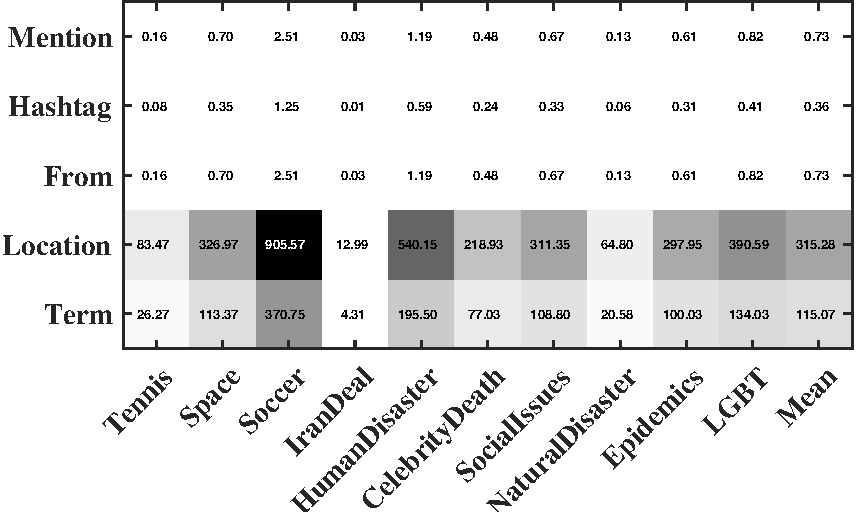
\includegraphics[width=0.5\textwidth]{images/medianMI.pdf}
%\vspace{-3mm}
%\caption{Median MI for different features vs. Topics, last two column show mean value and stderr across all topics}
%\label{fig:medianMI}
%\end{figure}
\begin{figure}[h!]
\centering
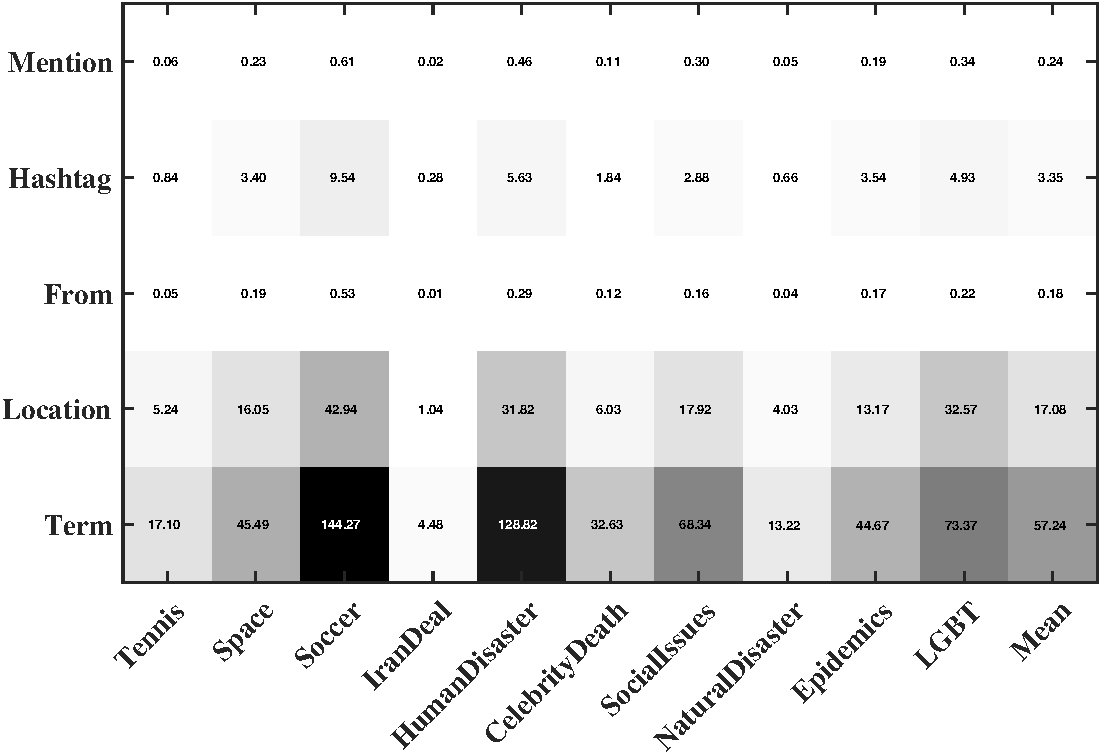
\includegraphics[width=0.5\textwidth]{images/avgMI_gray.pdf}
\vspace{-3mm}
\caption{Average MI for different features vs. Topics, last two column show mean value and stderr across all topics}
\label{fig:avgMI}
\end{figure}
%%%%%%%%%%%%%%%%%%%%%%%%%%%%%%%%%%%%%%%%%%%%%%%%%%%%%%%%%%%%%%%%%%%%%%%%%%%

%%%%%%%%%%%%%%%%%%%%%%%%%%%%%%%%%%%%%%%%%%%%%%%%%%%%%%%%%%%%%%%%%%
\begin{table*}[ht]
\centering
{\renewcommand{\arraystretch}{1.2}
\resizebox{\textwidth}{!}{%
\begin{tabular}{|l|l|l|l|l|l|l|l|l|l|l|}
\hline
\textbf{Topics/Top10} & \textbf{NaturalDisaster} & \textbf{Epidemics} & \textbf{IranDeal} & \textbf{SocialIssues} & \textbf{LBGT} & \textbf{HumanDisaster} & \textbf{CelebrityDeath} & \textbf{Space} & \textbf{Tennis} & \textbf{Soccer} \\ \hline
\textbf{From} & earthquake\_wo & changedecopine & mazandara & nsingerdebtpaid & eph4\_15 & ydumozyf & nmandelaquotes & daily\_astrodata & tracktennisnews & losangelessrh \\ \hline
\textbf{From} & earthalerts & drdaveanddee & hhadi119 & debtadvisoruk & mgdauber & syriatweeten & boiknox & freesolarleads & tennis\_result & shoetale \\ \hline
\textbf{From} & seelites & joinmentornetwk & 140iran & debt\_protect & stevendickinson & tintin1957 & jacanews & houston\_\_jobs & i\_roger\_federer & sport\_\_agent \\ \hline
\textbf{From} & globalfloodnews & followebola & setarehgan & negativeequityf & lileensvf1 & sirajsol & ewnreporter & star\_wars\_gifts & tennislessonnow & books\_you\_want \\ \hline
\textbf{From} & gcmcdrought & localnursejobs & akhgarshabaneh & dolphin\_ls & truckerbooman & rt3syria & paulretweet & lenautilus & kamranisbest & makeupbella \\ \hline \hline
\textbf{Hashtag} & earthquake & health & iran & ferguson & tcot & syria & rip & science & wimbledon & lfc \\ \hline
\textbf{Hashtag} & haiyan & uniteblue & irantalks & mikebrown & p2 & gaza & riprobinwilliams & starwars & usopen & worldcup \\ \hline
\textbf{Hashtag} & storm & ebola & rouhani & ericgarner & pjnet & isis & ripcorymonteith & houston & tennis & arsenal \\ \hline
\textbf{Hashtag} & tornado & healthcare & iranian & blacklivesmatter & uniteblue & israel & mandela & sun & nadal & worldcup2014 \\ \hline
\textbf{Hashtag} & prayforthephilippines & depression & no2rouhani & fergusondecision & teaparty & mh370 & nelsonmandela & sxsw & wimbledon2014 & halamadrid \\ \hline \hline
\textbf{Location} & philippines & usa & tehran & st.louis & usa & malaysia & southafrica & germany & london & liverpool \\ \hline
\textbf{Location} & ca & ncusa & u.s.a & mo & bordentown & palestine & johannesburg & roodepoort & uk & manchester \\ \hline
\textbf{Location} & india & garlandtx & nederland & usa & newjersey & syria & capetown & houston & india & london \\ \hline
\textbf{Location} & newdelhi & oh-sandiego & iran & dc & sweethomealabama! & israel & pretoria & austin & pakistan & nigeria \\ \hline
\textbf{Location} & newzealand & washington & globalcitizen & washington & aurora & london & durban & tx & islamabad & india \\ \hline \hline
\textbf{Mention} & oxfamgb & foxtramedia & 4freedominiran & deray & jjauthor & ifalasteen & nelsonmandela & bizarro\_chile & wimbledon & lfc \\ \hline
\textbf{Mention} & weatherchannel & obi\_obadike & iran\_policy & natedrug & 2anow & revolutionsyria & realpaulwalker & nasa & usopen & arsenal \\ \hline
\textbf{Mention} & redcross & who & hassanrouhani & antoniofrench & govchristie & drbasselabuward & robinwilliams & j\_ksen & andy\_murray & realmadriden \\ \hline
\textbf{Mention} & twcbreaking & obadike1 & un & bipartisanism & a5h0ka & mogaza & rememberrobin & jaredleto & serenawilliams & ussoccer \\ \hline
\textbf{Mention} & abc7 & c25kfree & statedept & theanonmessage & barackobama & palestinianism & tweetlikegiris & 30secondstomars & espntennis & mcfc \\ \hline \hline
\textbf{Term} & philippines & health & iran & police & obama & israel & robin & cnblue & murray & madrid \\ \hline
\textbf{Term} & donate & ebola & regime & protesters & gun & gaza & williams & movistar & tennis & goal \\ \hline
\textbf{Term} & typhoon & acrx & nuclear & officer & rights & israeli & nelson & enero & federer & cup \\ \hline
\textbf{Term} & affected & medical & iranian & protest & america & killed & mandela & ΍imperdible & djokovic & manchester \\ \hline
\textbf{Term} & relief & virus & resistance & cops & gop & children & cory & greet & nadal & match \\ \hline
\end{tabular}
}}
\caption{Top 5 features for each topic based on Mutual Information}
\label{table:top10MItopicsLocations}
\end{table*}
%%%%%%%%%%%%%%%%%%%%%%%%%%%%%%%%%%%%%%%%%%%%%%%%%%%%%%%%%%%%%%%%%%
In order to answer the second question on whether any attributes correlate with importance for each feature, we provide two set of analysis. The first one, provides Mutual Information values of each feature across feature's attribute values shown by violin plots in figure \ref{fig:violinplots}. The attributes for each feature are:

\begin{itemize}
\item From: favorite count (the number of tweets the user has favorited), followers count (the number of users who follow the user), friends count (the number of users followed by the user), hashtag count (number of hashtags used by the user), tweet count (the number of tweets from the user)
\item Hashtag: tweet count, user count (the number of users using the hashtag)
\item Location: user count
\item Mention: tweet count
\item Term: tweet count
\end{itemize}

As we can see in the violin plots, the general pattern is that the more number of tweets, users, or hashtags count a feature has, the higher the chance of becoming topical will be. This pattern exists on other attributes of $From$ feature, although a bit less clear than the tweets, users, or hashtags counts attributes. 
In addition, we further analyzed the density plots of favorite count, follower count, friends count, hashtag count attributes of $From$ feature shown in Fig ~\ref{fig:densityplots}. These plots represent a bi-modality in the distribution. Further analysis of data showed that the top mode belongs to users who have at least one topical tweet while bottom mode are users with no topical tweet.

%%%%%%%%%%%%%%%%%%%%%%%%%%%%%%%%%%%%%%%%%%%%%%%%%%%%%%%%%%%%%%%%%%%%%%%%%%%
\iffalse
\begin{figure*}[th!]
\centering
\begin{tabular}{ccccc}
\begin{tabular}{ccccc}
\subfloat[Fig:][Favorite Count]{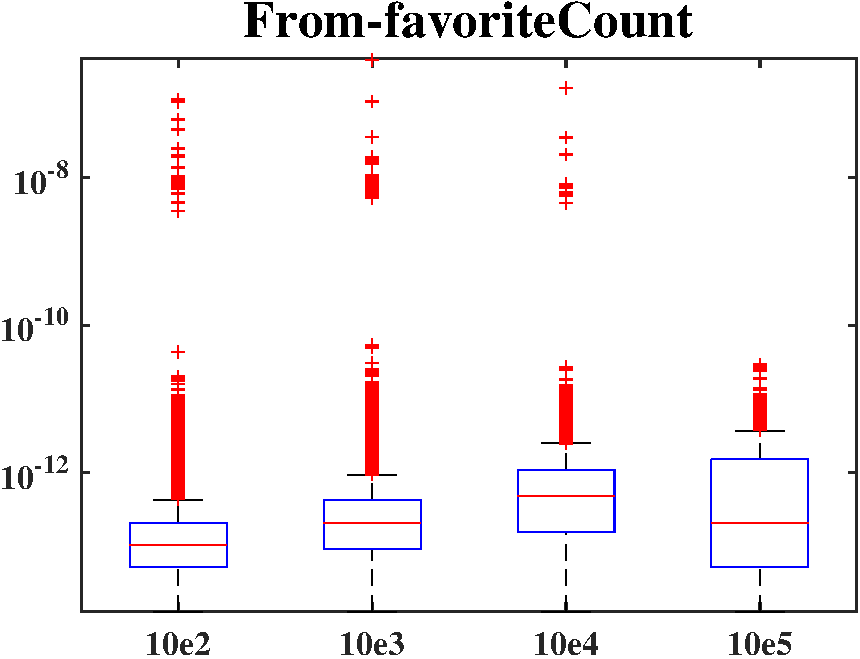
\includegraphics[width=32mm, height=35mm]{images/BoxPlots_IranDeal/From-favoriteCount.pdf}}
\subfloat[Fig:][Followers Count]{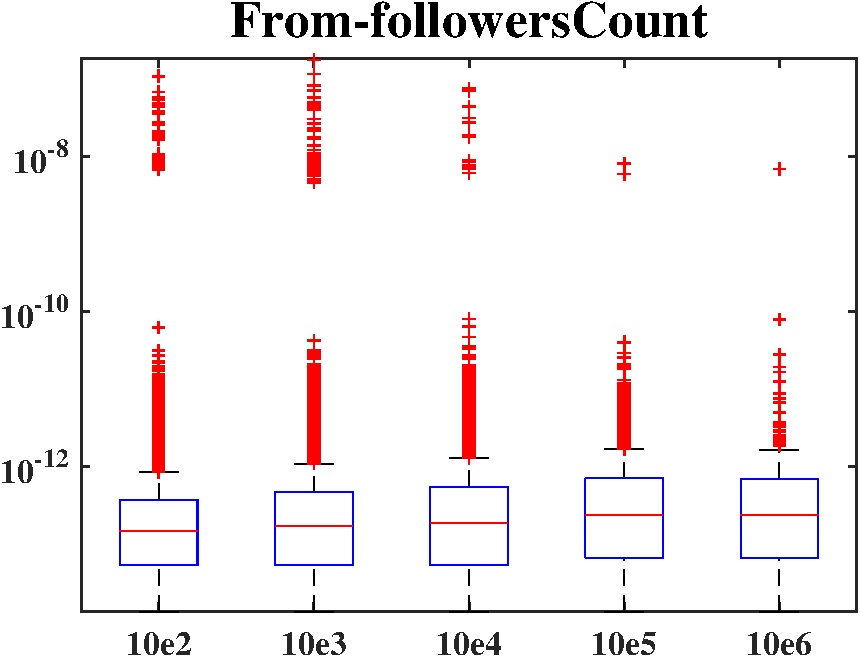
\includegraphics[width=32mm, height=35mm]{images/BoxPlots_IranDeal/From-followersCount.pdf}}
\subfloat[Fig:][Friends Count]{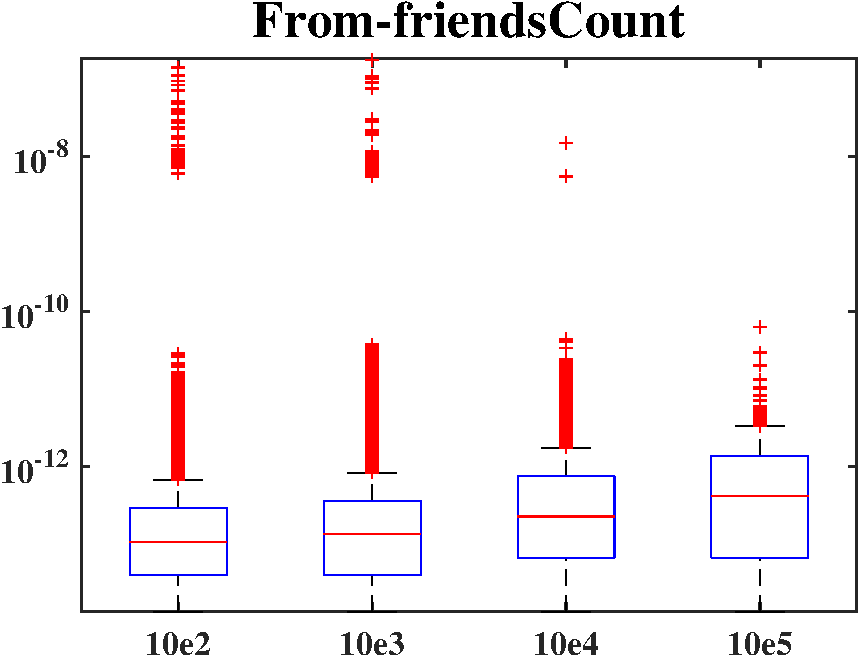
\includegraphics[width=32mm, height=35mm]{images/BoxPlots_IranDeal/From-friendsCount.pdf}}
\subfloat[Fig:][Hashtag Count]{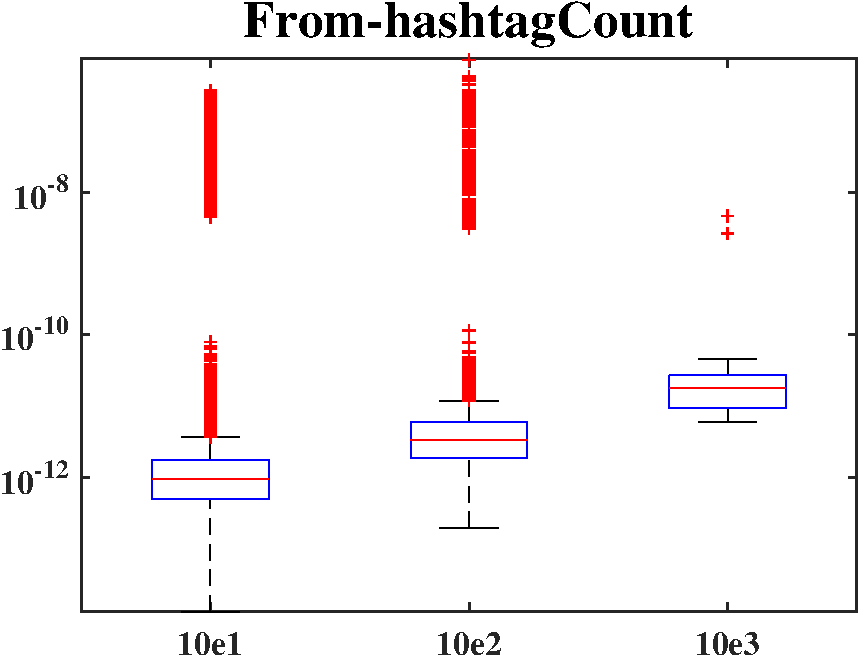
\includegraphics[width=32mm, height=35mm]{images/BoxPlots_IranDeal/From-hashtagCount.pdf}}
\subfloat[Fig:][Tweet Count]{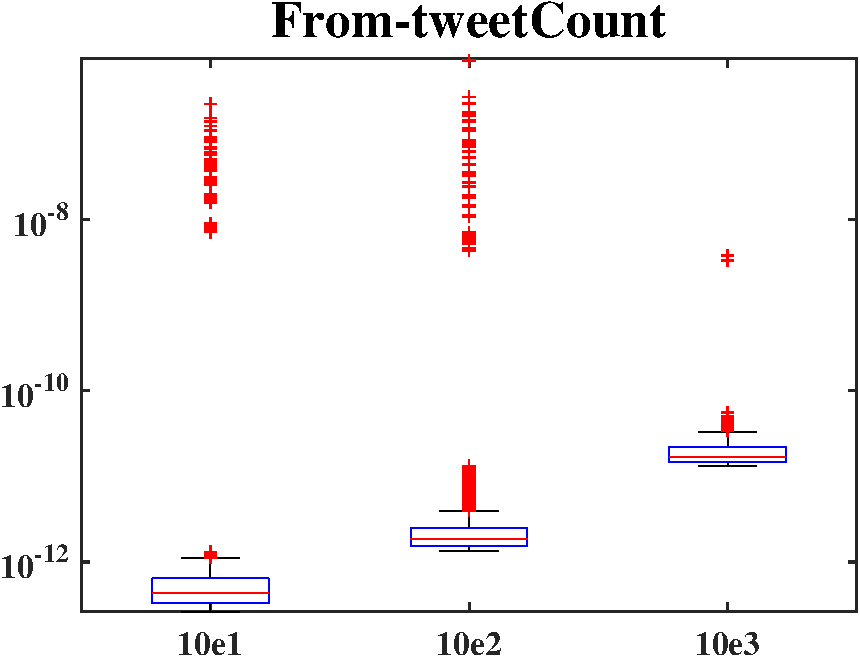
\includegraphics[width=32mm, height=35mm]{images/BoxPlots_IranDeal/From-tweetCount.pdf}} \\
%\vspace{-10mm}
\subfloat[Fig:][Tweet Count]{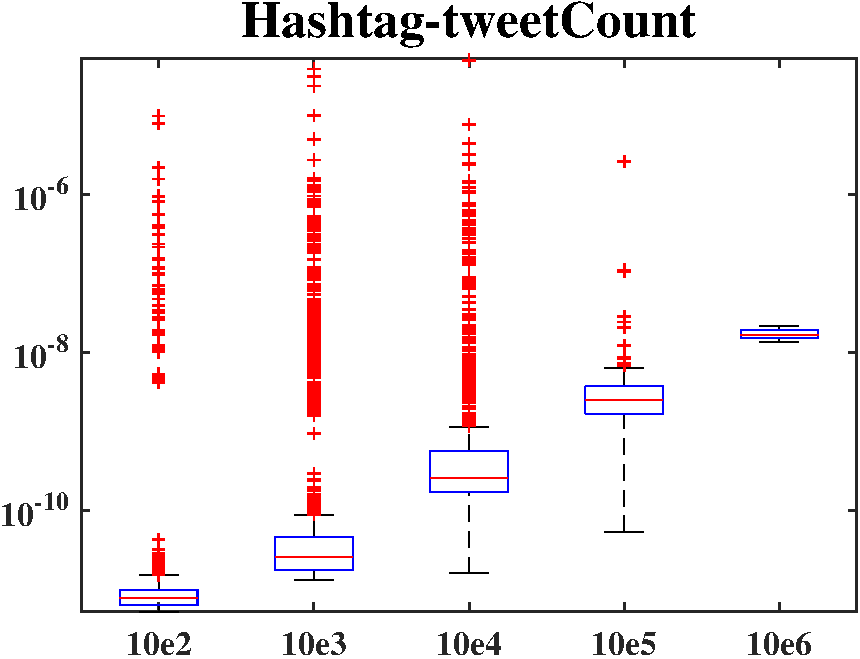
\includegraphics[width=32mm, height=35mm]{images/BoxPlots_IranDeal/Hashtag-tweetCount.pdf}}
\subfloat[Fig:][User Count]{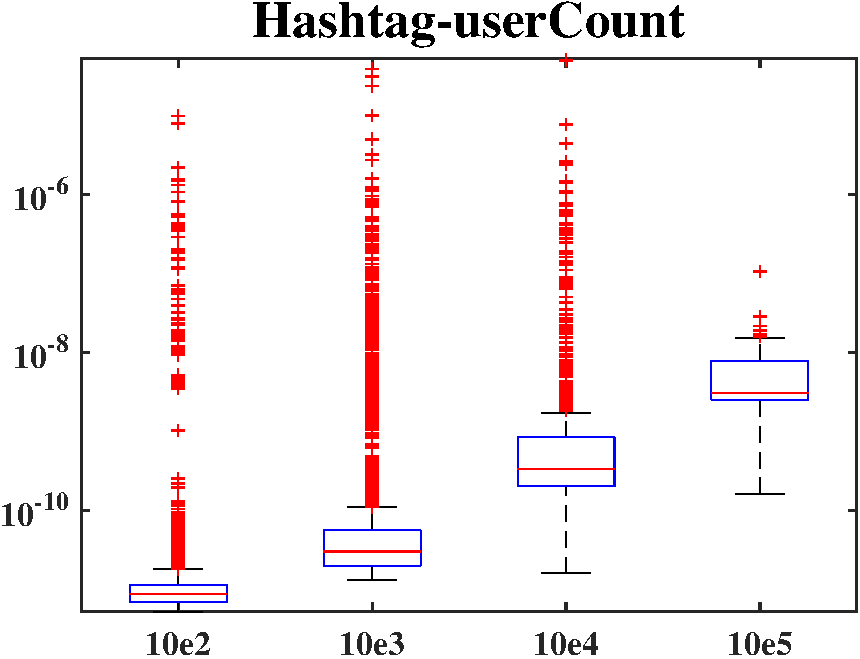
\includegraphics[width=32mm, height=35mm]{images/BoxPlots_IranDeal/Hashtag-userCount.pdf}}
\subfloat[Fig:][User Count]{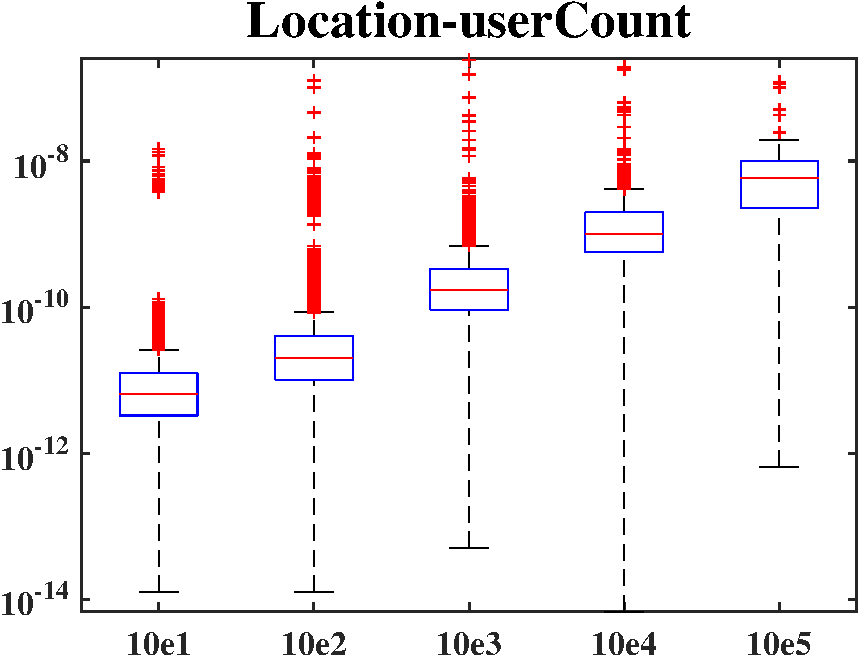
\includegraphics[width=32mm, height=35mm]{images/BoxPlots_IranDeal/Location-userCount.pdf}}
\subfloat[Fig:][Tweet Count]{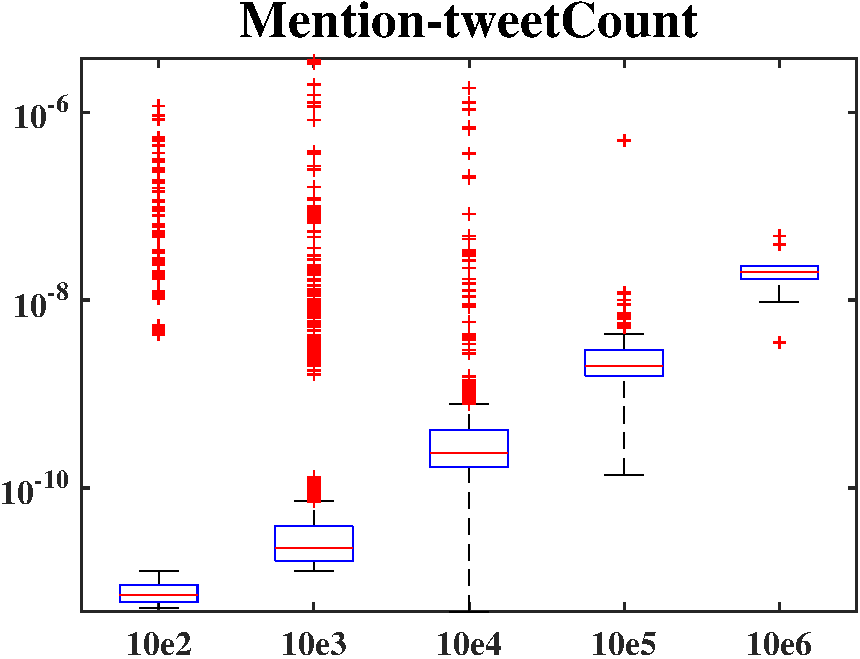
\includegraphics[width=32mm, height=35mm]{images/BoxPlots_IranDeal/Mention-tweetCount.pdf}}
\subfloat[Fig:][Tweet Count]{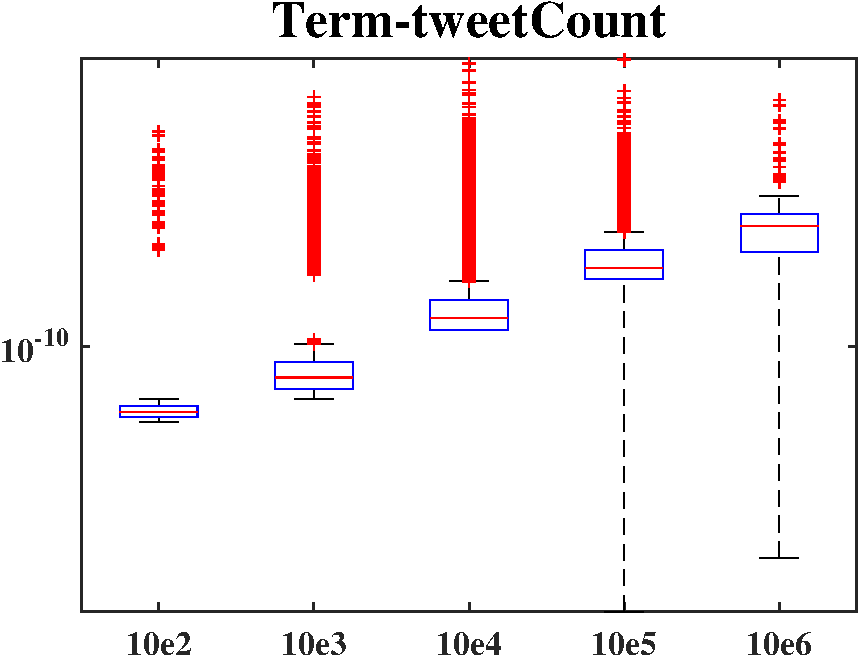
\includegraphics[width=32mm, height=35mm]{images/BoxPlots_IranDeal/Term-tweetCount.pdf}} \\
\end{tabular}
\end{tabular}
\vspace{-2mm}
\caption {Box Plots for feature attributes counts vs. MI. Top row shows attributes \{favoriteCount, followerCount, friendCount, hashtagCount, tweetCount\} for $From$ feature. Bottom row shows attributes tweetCount and/or userCount for $Hashtag$, $Location$, $Mention$,and $Term$ features.}
\label{fig:boxplots2}
\end{figure*}
\fi
%%%%%%%%%%%%%%%%%%%%%%%%%%%%%%%%%%%%%%%%%%%%%%%%%%%%%%%%%%%%%%%%%%%%%%%%%%%


%%%%%%%%%%%%%%%%%%%%%%%%%%%%%%%%%%%%%%%%%%%%%%%%%%%%%%%%%%%%%%%%%%%%%%%%%%%
\begin{figure*}[tph!]
\centering
\begin{tabular}{ccccc}
\begin{tabular}{ccccc}
\subfloat[Fig:][]{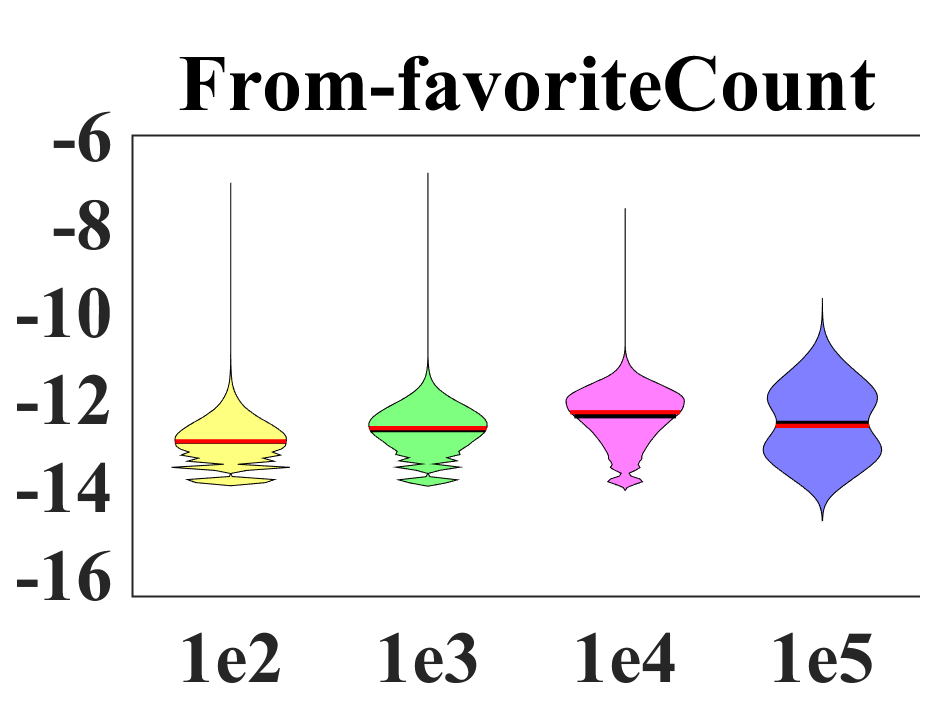
\includegraphics[width=32mm, height=35mm]{images/ViolinPlots/From-favoriteCount.eps}}
\subfloat[Fig:][]{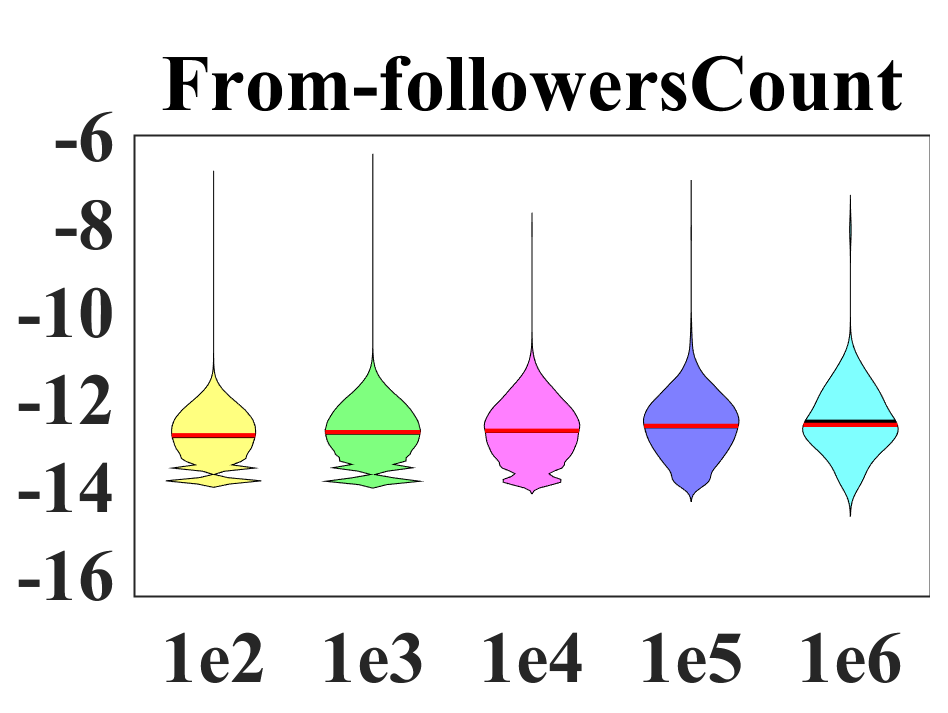
\includegraphics[width=32mm, height=35mm]{images/ViolinPlots/From-followersCount.eps}}
\subfloat[Fig:][]{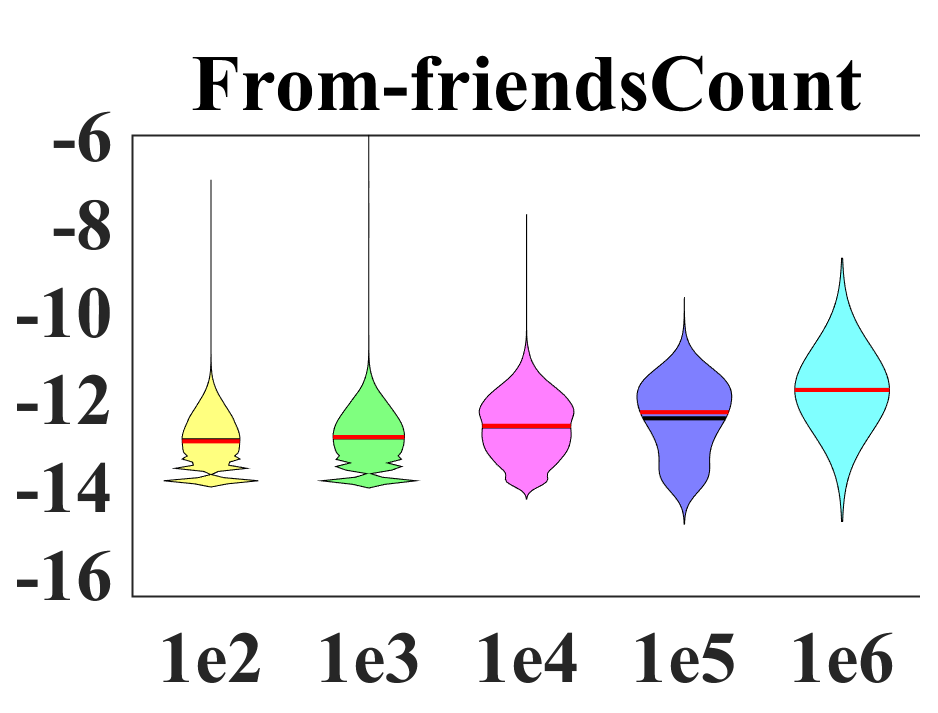
\includegraphics[width=32mm, height=35mm]{images/ViolinPlots/From-friendsCount.eps}}
\subfloat[Fig:][]{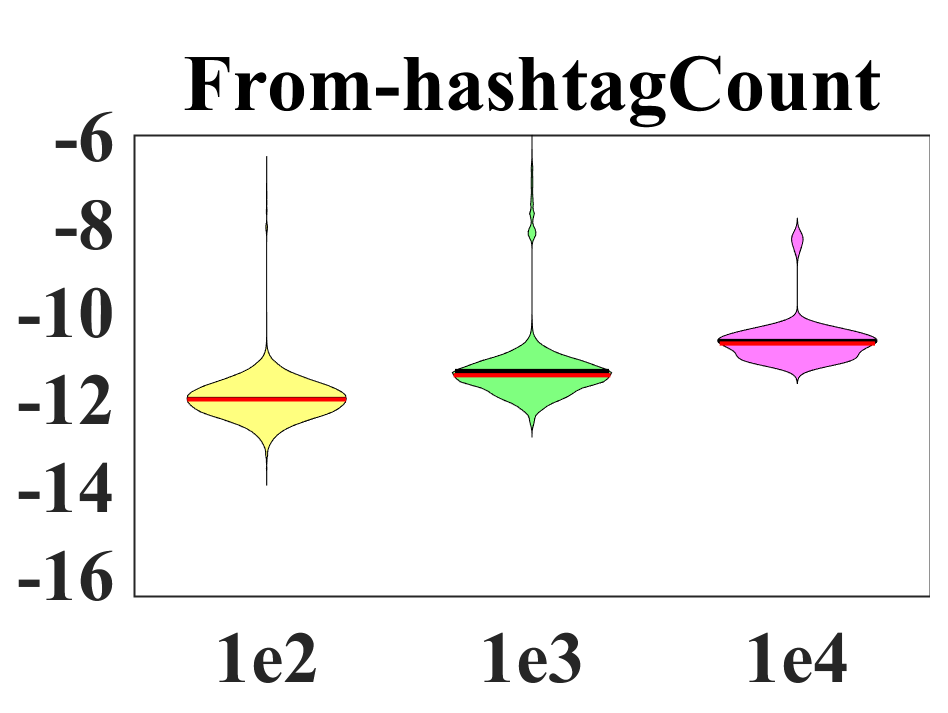
\includegraphics[width=32mm, height=35mm]{images/ViolinPlots/From-hashtagCount.eps}}
\subfloat[Fig:][]{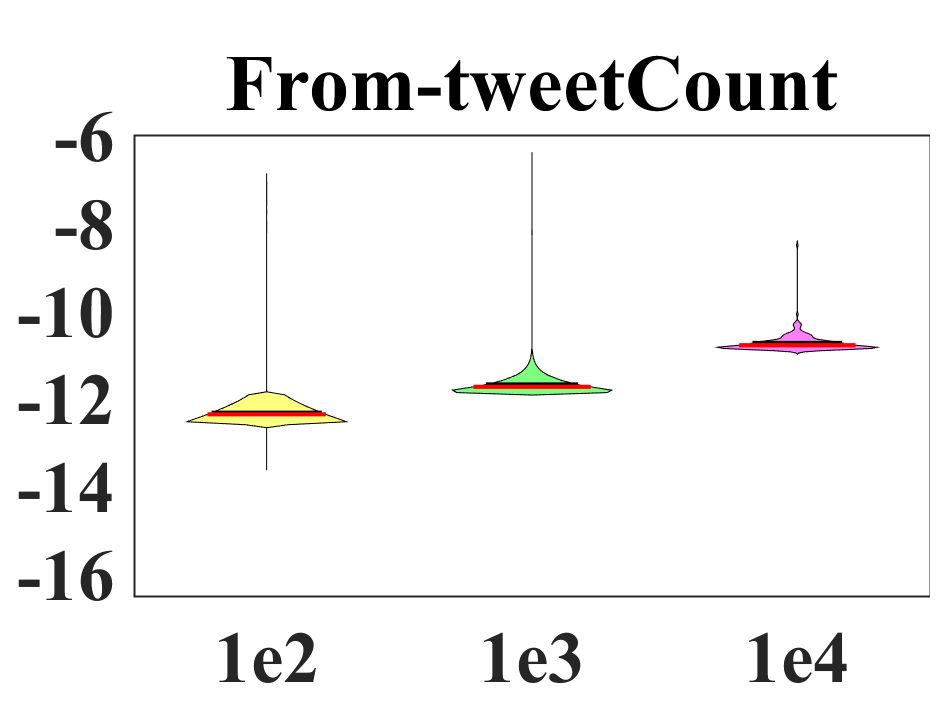
\includegraphics[width=32mm, height=35mm]{images/ViolinPlots/From-tweetCount.eps}} \\
%\vspace{-10mm}
\subfloat[Fig:][]{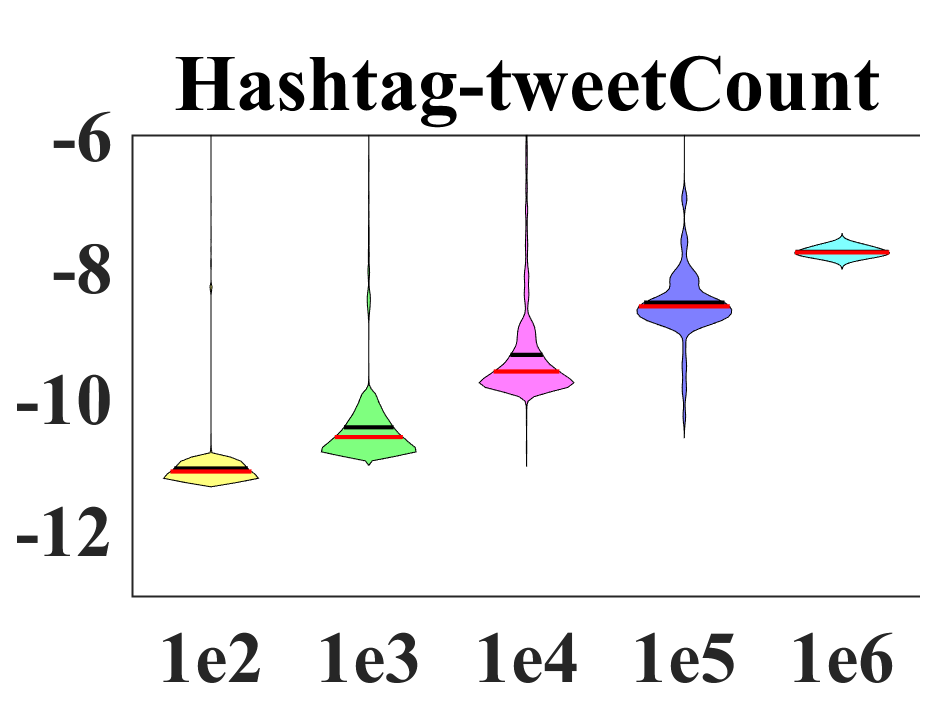
\includegraphics[width=32mm, height=35mm]{images/ViolinPlots/Hashtag-tweetCount.eps}}
\subfloat[Fig:][]{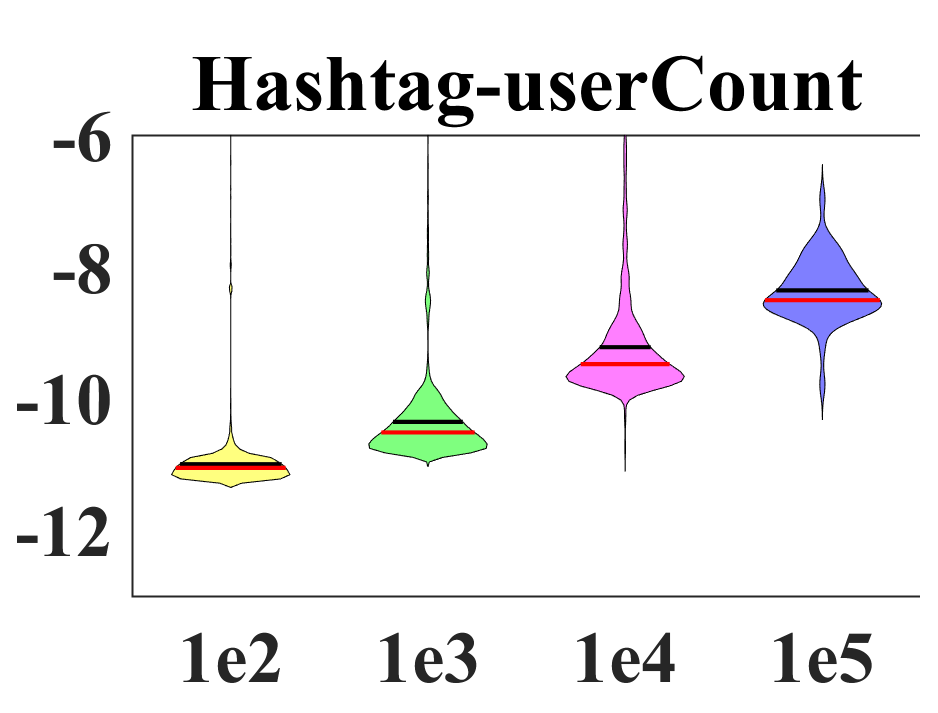
\includegraphics[width=32mm, height=35mm]{images/ViolinPlots/Hashtag-userCount.eps}}
\subfloat[Fig:][]{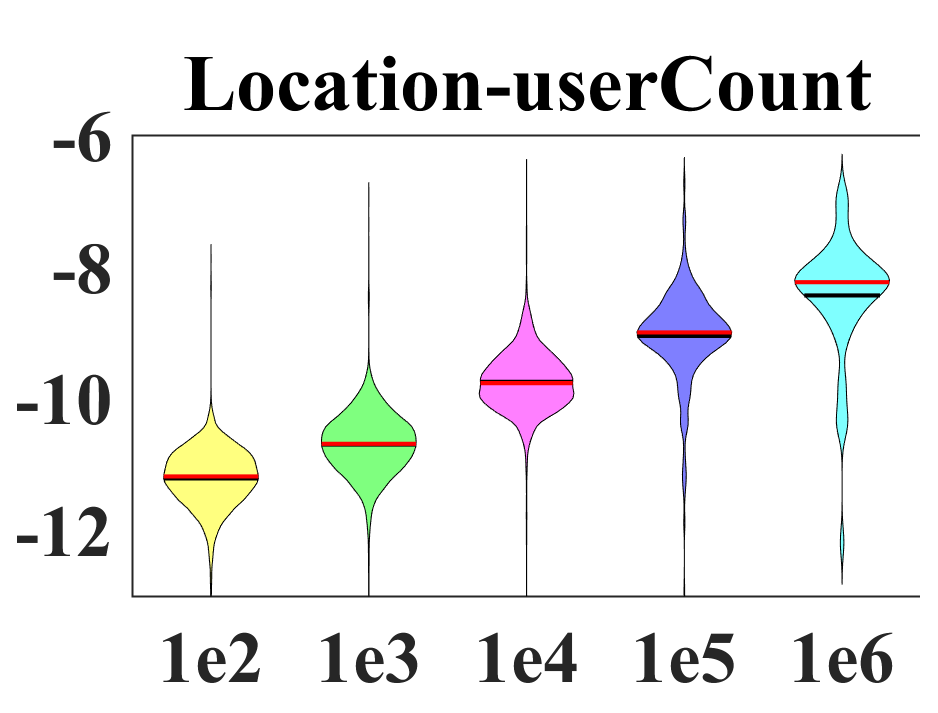
\includegraphics[width=32mm, height=35mm]{images/ViolinPlots/Location-userCount.eps}}
\subfloat[Fig:][]{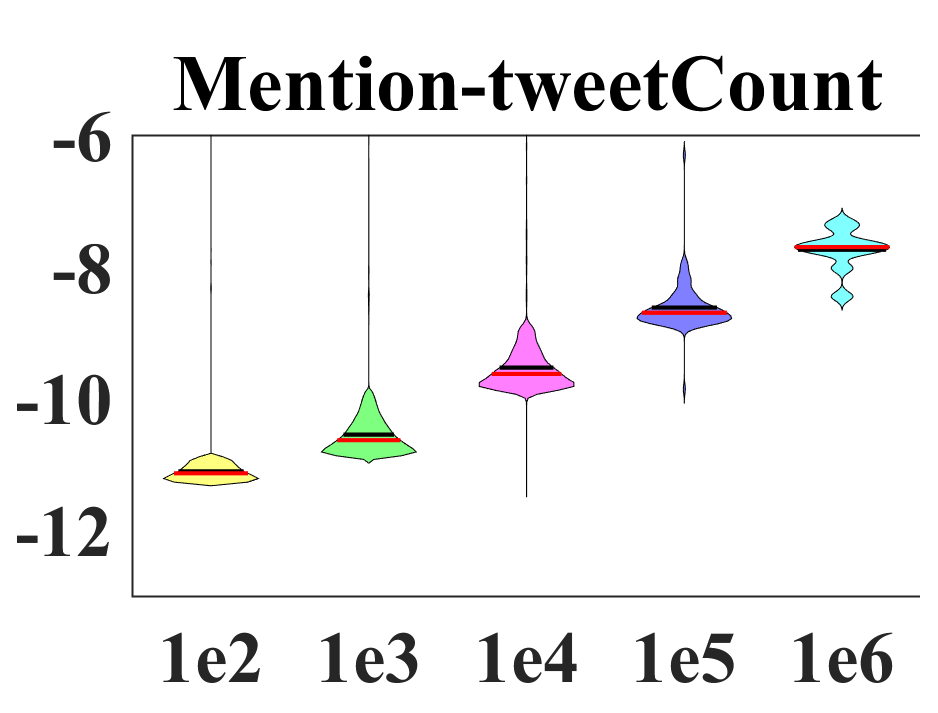
\includegraphics[width=32mm, height=35mm]{images/ViolinPlots/Mention-tweetCount.eps}}
\subfloat[Fig:][]{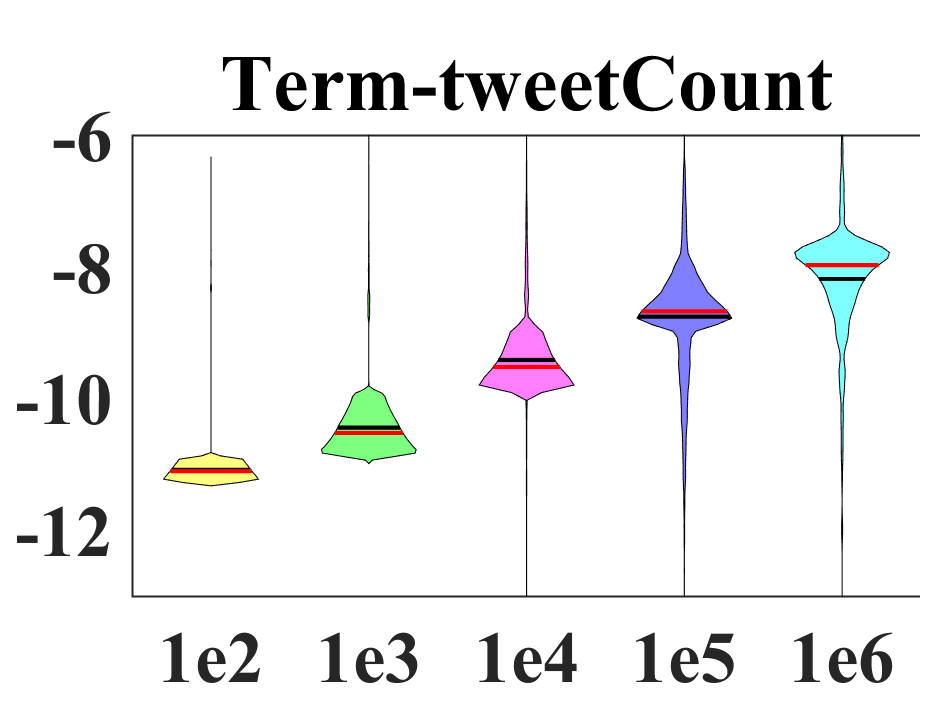
\includegraphics[width=32mm, height=35mm]{images/ViolinPlots/Term-tweetCount.eps}} \\
\end{tabular}
\end{tabular}
\vspace{-2mm}
\caption {ViolinPlots for feature attributes counts vs. MI. Top row shows attributes \{favoriteCount, followerCount, friendCount, hashtagCount, tweetCount\} for $From$ feature. Bottom row shows attributes tweetCount and/or userCount for $Hashtag$, $Location$, $Mention$,and $Term$ features.}
\label{fig:violinplots}
\end{figure*}
%%%%%%%%%%%%%%%%%%%%%%%%%%%%%%%%%%%%%%%%%%%%%%%%%%%%%%%%%%%%%%%%%%%%%%%%%%%


%%%%%%%%%%%%%%%%%%%%%%%%%%%%%%%%%%%%%%%%%%%%%%%%%%%%%%%%%%%%%%%%%%%%%%%%%%%
\begin{figure*}[tbh!]
\centering
\begin{tabular}{cccc}
\subfloat[Fig:][]{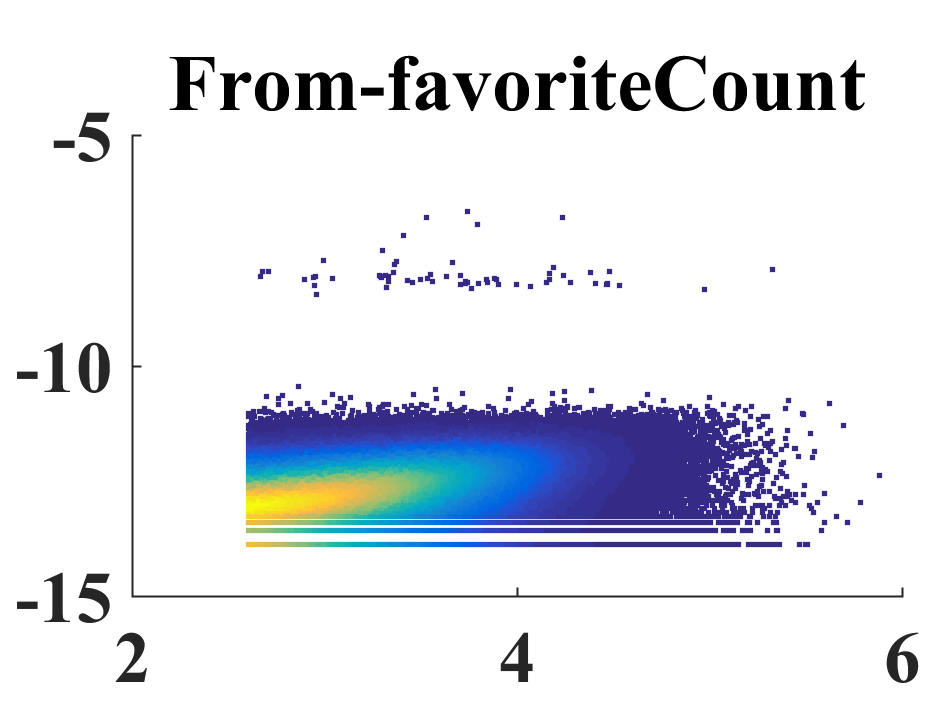
\includegraphics[width=40mm, height=35mm]{images/DensityPlots_IranDeal/dscatterPlot_From-favoriteCount.eps}} \qquad
\subfloat[Fig:][]{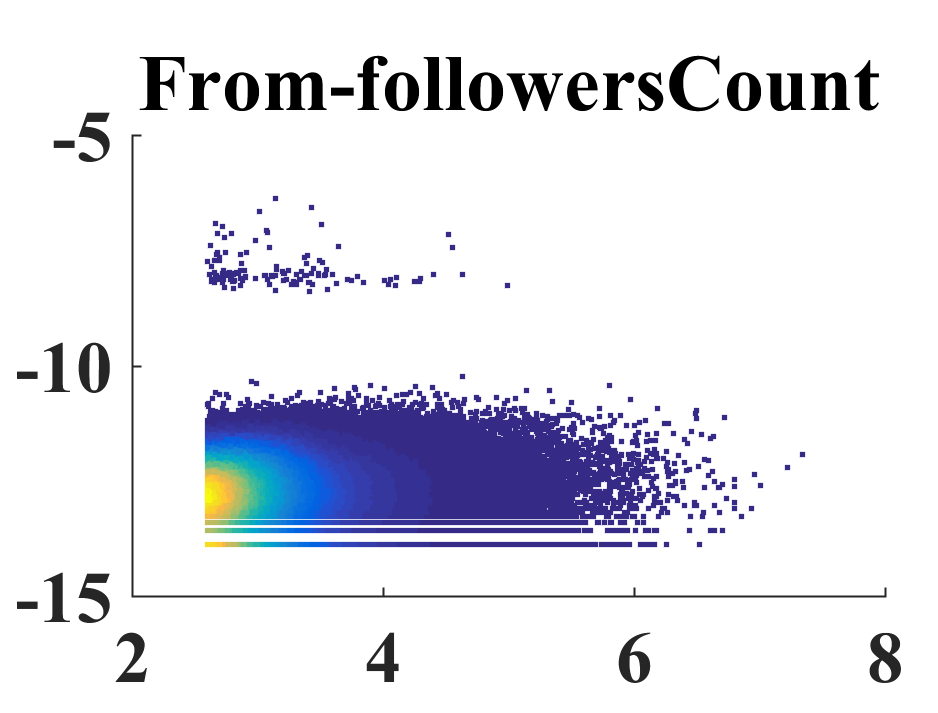
\includegraphics[width=40mm, height=35mm]{images/DensityPlots_IranDeal/dscatterPlot_From-followersCount.eps}} \qquad
\subfloat[Fig:][]{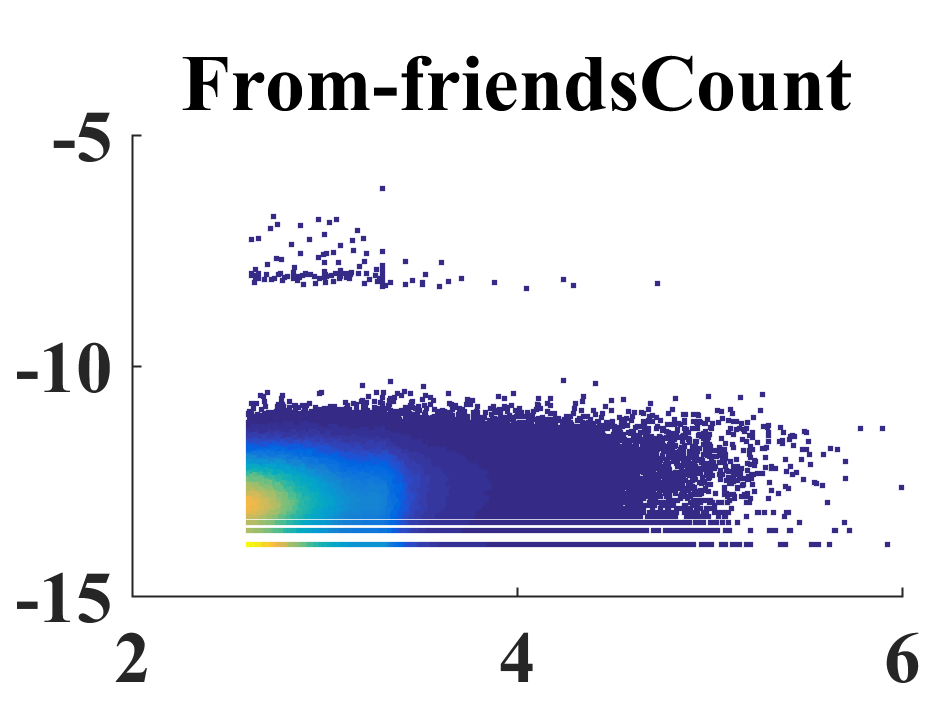
\includegraphics[width=40mm, height=35mm]{images/DensityPlots_IranDeal/dscatterPlot_From-friendsCount.eps}} \qquad
\subfloat[Fig:][]{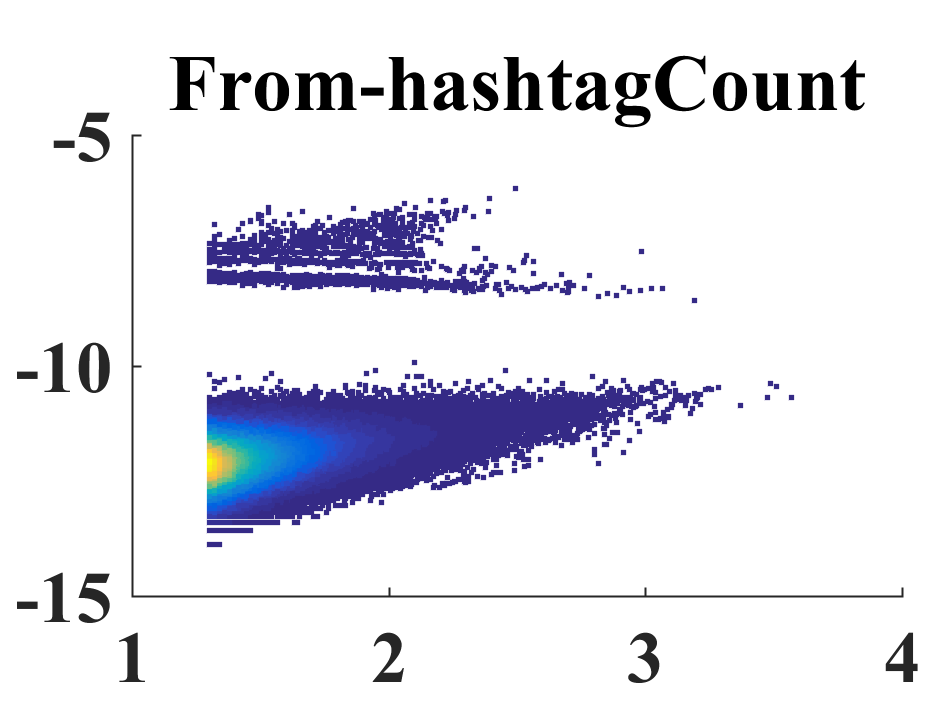
\includegraphics[width=40mm, height=35mm]{images/DensityPlots_IranDeal/dscatterPlot_From-hashtagCount.eps}} \\
\end{tabular}
\vspace{-2mm}
\caption {DensityPlots for feature attributes counts vs. MI. (a-d) show attributes \{favoriteCount, followerCount, friendCount, hashtagCount\} for $From$ feature}
\label{fig:densityplots}
\end{figure*}
%%%%%%%%%%%%%%%%%%%%%%%%%%%%%%%%%%%%%%%%%%%%%%%%%%%%%%%%%%%%%%%%%%

\section{Conclusions and Future Work}
This work fills a major gap in 
event detection and tracking from social media
on identifying emerging topics from long-running themes with
minimal user supervision.  
We contribute a novel supervised method for training social sensors with minimal user curation by using a small seed set of hashtags as topical proxies for automatic supervised data labeling. The supervised classification and ranking methods learn topical content from a large feature space. We train our social sensor on known topical content, but tune it on novel topical validation content which ensures optimal generalization. The experiments are on a corpus of over $800$ million tweets crawled with Twitter Search API. Our results suggest that these
sensors generalize well to unseen future topical content and provide a
novel paradigm for the extraction of high-value content from social
media. Furthermore, we provide an
extensive analysis of features and feature attributes across different
topics that reveals, (1)~largely independent of
topic, simple terms are the most informative feature followed by
location features and that (2)~the number of unique hashtags and
tweets by a user correlates more with their informativeness than their follower or friend count.

Future work should explore the following enhanced topical
social sensor learning tasks: (1) optimizing rankings not only for topicality
but also to minimize the lag-time of novel content identification, (2) optimizing
queries for boolean retrieval oriented APIs such as Twitter, and (3) utilizing 
more social network structure to exploit a more expressive graph-based features.


\section{Extra}
% Contribution 
% 1. What do we offer? Combing recent ideas, expand, offer more
% 2. What was the previous ideas? 
%      2.1. Automatic labeling of lots of tweets, 
%      2.2. Using learning methodologies for detection of general topical content
% 3. How did we build on these ideas?
% 4: What do we offer in addition to combination.
\subsection*{Discussion of Contributions}
In this work, we coalesce recent ideas on learning social sensors for general topic detection. We expand these works to learn a generalizable supervised method with minimal user curation for detecting and ranking topical content over a variety of topics and on a long-term dataset. We believe that no earlier work covers all the aspects of the work presented here.
Earlier works discuss leveraging learning methodologies for detection of topical content from social media for general topics ~\cite{lin2011smoothing,yang2014large,magdy}. One of the key challenges of using learning methods for general topics and large number of tweets is automatic labeled data aquisition. To this purpose~\cite{lin2011smoothing} discuss automatic labeling of tweets by using one hashtag as topic proxy.~\cite{magdy} use a user-defined query to label tweets and~\cite{yang2014large} take a co-training approach based on embedded URLs in the tweet and tweet text to label tweets. We build and extend on~\cite{lin2011smoothing}'s idea of automatic labeling of tweets, however we choose a \emph{set} of hashtags for each topic instead of a single hashtag which we will show to be imperative for evaluating generalization. To learn social sensors for general topic detection,~\cite{lin2011smoothing} use information retrieval method (language models),~\cite{yang2014large} take advantage of topic modeling techniques and~\cite{magdy} apply SVM classifier. Here, we leverage more than one supervised learning method for the purpose of detection and ranking of topical content. We present a unique method for splitting hashtags and Twitter data that encourages generalization to new unseen future content. 

%%%%% TRACKING GENERAL TOPICS
\subsection*{Tracking General Topics} 
represents use of social media sensors for detecting and tracking general topics such as "Baseball" and "Fashion". Researchers have collected labeled data by using a single hashtag for each topic~\cite{lin2011smoothing}, a user-defined query for each topic~\cite{magdy}, or co-training based on the URLs and text of the tweet~\cite{yang2014large}.~\cite{lin2011smoothing} leverages language models to train models using unigrams and bigrams,~\cite{magdy} applies SVM classifier on extracted hashtags, unigrams, users and mentions as features, and~\cite{yang2014large} defines the problem as topic modeling of tweets. We expand on~\cite{lin2011smoothing}'s work and use a set of hashtags instead of a single hashtag. We extract hashtags, mentions, unigrams, users as features inline with these works. However, we add location as another feature which we will show later that location is the second most important feature for detection of topical content. We take advantage of various supervised learning methods and provide a novel framework for learning in terms of splitting the data and hashtags as topical proxies that would ensure generalization to future unseen content. While these works provide a good basis for this work, there are many fine-grain but important differences between previous works and this work with the most important ones being:
\begin{enumerate}
\item We analyzed long-term sensor performance on detecting topical content over two years of Twitter data and across a variety of topics.
\item We provide a novel and clear framework for splitting hashtags to train, validation and test in a way ensuring generalization to future unseen content.
\item We present ranking in addition to correct classification while none of the other works provide ranking.
\item We deliver a comprehensive longitudinal study on features and their attributes over two years of tweets that supports our insights for learning and relevance of features to topicality while these works had little or none analysis over their features.
\item We extract \textit{Location} as one of the features which none of these works do and as we show in our feature analysis, \textit{Location} is the second most important feature beating even hashtags in terms of correlation with topicality.
\end{enumerate}


% No identifying information in submitted version. -SPS
%\section{Acknowledgments}
%acknowledgements
%
%\section{Copyright}

\bibliographystyle{aaai}
\bibliography{bibliography}

\end{document}
